\documentclass[11pt,a4paper]{article}

\usepackage[T1]{fontenc}
\usepackage[french]{babel}
\usepackage{lmodern}
\usepackage{microtype}
\usepackage[a4paper,top=2.5cm,bottom=2.5cm,left=2.4cm,right=2.4cm,headheight=14pt]{geometry}
\usepackage{graphicx}
\usepackage{booktabs}
\usepackage{multirow}
\usepackage{array}
\usepackage{tabularx}
\usepackage{makecell}
\usepackage{float}
\usepackage[table]{xcolor}
\usepackage{amsmath}
\usepackage{amssymb}
\usepackage{icomma}
\usepackage{enumitem}
\usepackage{fancyhdr}
\usepackage{titlesec}
\usepackage[font=small,labelfont=bf,labelsep=period]{caption}
\usepackage{subcaption}
\usepackage{csquotes}
\usepackage{tikz}
\usetikzlibrary{arrows.meta,positioning,shapes.geometric,fit,backgrounds,calc,babel}
\usepackage[backend=biber,style=numeric-comp,sorting=none,maxbibnames=4,minbibnames=3,giveninits=true,isbn=false,eprint=false,url=true,doi=true]{biblatex}
\usepackage{xurl}
\usepackage[colorlinks=true,linkcolor=accent,citecolor=accent,urlcolor=accent]{hyperref}

\addbibresource{references.bib}
\DeclareSourcemap{
  \maps[datatype=bibtex]{
    \map[overwrite]{
      \step[fieldsource=doi, final]
      \step[fieldset=url, null]
    }
  }
}
\graphicspath{{figures/}}

\makeatletter
\newcommand{\tableinput}[1]{\@@input #1 }
\makeatother

\definecolor{accent}{HTML}{1C5CAB}
\definecolor{lightaccent}{HTML}{CDE2FB}
\definecolor{softgray}{HTML}{F0EFEC}
\definecolor{inkgray}{HTML}{52514E}

\newcommand{\depot}{\url{https://github.com/Abderrahmane-Elhouij/sugarcane-leaf-disease-classification}}

\renewcommand{\thesection}{\Roman{section}}
\renewcommand{\thesubsection}{\thesection.\arabic{subsection}}
\renewcommand{\thesubsubsection}{\thesubsection.\arabic{subsubsection}}
\titleformat{\section}{\Large\bfseries\color{accent}}{\thesection.}{0.6em}{}
\titleformat{\subsection}{\large\bfseries}{\thesubsection}{0.7em}{}
\titleformat{\subsubsection}{\normalsize\bfseries}{\thesubsubsection}{0.7em}{}
\titlespacing*{\section}{0pt}{1.6em}{0.9em}
\titlespacing*{\subsection}{0pt}{1.2em}{0.6em}
\setcounter{secnumdepth}{3}
\setcounter{tocdepth}{2}

\setlist{itemsep=0.25em,topsep=0.4em}
\renewcommand{\arraystretch}{1.15}
\setlength{\parskip}{0.35em}

\pagestyle{fancy}
\fancyhf{}
\fancyhead[L]{\small\color{inkgray} Classification des maladies foliaires de la canne à sucre}
\fancyhead[R]{\small\color{inkgray} Master ISI -- FSSM}
\fancyfoot[C]{\small \thepage}
\renewcommand{\headrulewidth}{0.4pt}

\begin{document}

\begin{titlepage}
\thispagestyle{empty}
\centering

\includegraphics[width=0.40\textwidth]{logo_fssm.png}\par
\vspace{0.5cm}
{\large Université Cadi Ayyad\par}
{\large Faculté des Sciences Semlalia -- Marrakech\par}
\vspace{0.15cm}
{\normalsize Département d'Informatique\par}
\vspace{0.15cm}
{\normalsize Master ISI -- Semestre 3 \quad\textbullet\quad Module : Deep Learning (Transfer Learning)\par}

\vspace{2.2cm}
{\color{accent}\rule{\textwidth}{1pt}}\par
\vspace{0.5cm}
{\LARGE\bfseries Classification automatique des maladies des feuilles de canne à sucre par apprentissage profond et fusion de caractéristiques\par}
\vspace{0.5cm}
{\large Extraction de caractéristiques, fine-tuning partiel et fine-tuning complet\par}
\vspace{0.5cm}
{\color{accent}\rule{\textwidth}{1pt}}\par
\vspace{0.6cm}
{\large Rapport du projet n\textsuperscript{o}\,8\par}

\vfill
\begin{minipage}[t]{0.46\textwidth}
\raggedright
{\large\textbf{Réalisé par :}}\par
\vspace{0.2cm}
{\large Abderrahmane EL-HOUIJ}
\end{minipage}
\hfill
\begin{minipage}[t]{0.46\textwidth}
\raggedleft
{\large\textbf{Encadré par :}}\par
\vspace{0.2cm}
{\large Pr. Mustapha AATILA}
\end{minipage}

\vfill
{\large Année universitaire 2026--2027\par}
\end{titlepage}


\pagenumbering{roman}
\section*{Résumé}
\addcontentsline{toc}{section}{Résumé}

Les maladies foliaires de la canne à sucre réduisent fortement les rendements, et leur diagnostic repose encore largement sur l'inspection visuelle. Ce projet évalue l'apprentissage par transfert pour reconnaître automatiquement, à partir de photos prises au champ, quatre maladies (mosaïque, pourriture rouge, rouille et maladie de la feuille jaune) et les feuilles saines. Nous utilisons le jeu public de Daphal et Koli (2\,521 images, cinq classes), dont l'audit a révélé 210 doublons exacts et 24 quasi-doublons, supprimés avant tout découpage. Quatre architectures pré-entraînées sur ImageNet (EfficientNetV2-S, MobileNetV4-Conv-M, ConvNeXtV2-T et SE-ResNet-50) sont comparées selon trois stratégies, l'extraction de caractéristiques, le fine-tuning partiel et le fine-tuning complet, ainsi qu'à un CNN entraîné from scratch, dans des conditions identiques, avec un ensemble de test isolé et une validation croisée stratifiée à cinq plis. Nous étudions aussi la fusion des embeddings des quatre réseaux, sur les 15 combinaisons possibles, et un vote souple. Le fine-tuning complet l'emporte pour toutes les architectures : ConvNeXtV2-T atteint $98{,}9 \pm 0{,}6$\,\% d'accuracy (F1 macro de 98,9\,\%), contre 94,3\,\% pour le CNN from scratch et 83,9 à 90,8\,\% en extraction de caractéristiques. La fusion des modèles fine-tunés porte l'accuracy à 99,4\,\%, un gain modeste mais significatif. ConvNeXtV2-T est aussi le modèle unique le plus robuste aux dégradations d'image, et MobileNetV4-M offre le meilleur compromis pour un téléphone (97,9\,\% avec 8,4 millions de paramètres). Avec un quart seulement des images d'apprentissage, ConvNeXtV2-T (96,7\,\%) fait déjà mieux que le CNN from scratch entraîné sur la totalité. Les cartes Grad-CAM montrent enfin qu'après fine-tuning, les modèles s'appuient sur les lésions plutôt que sur l'arrière-plan.

\medskip
\noindent\textbf{Mots-clés :} canne à sucre ; maladies foliaires ; apprentissage par transfert ; fine-tuning ; fusion de caractéristiques ; Grad-CAM.

\medskip
\noindent\textbf{Code source du projet :} \depot

\section*{Abstract}
\addcontentsline{toc}{section}{Abstract}

\begin{otherlanguage}{english}
Leaf diseases cause major yield losses in sugarcane, and their diagnosis still relies mostly on visual inspection. This project evaluates transfer learning for recognising four diseases (mosaic, red rot, rust and yellow leaf disease) and healthy leaves from field photographs. We use the public dataset of Daphal and Koli (2,521 images, five classes); an audit revealed 210 exact duplicates and 24 near-duplicates, which were removed before any split. Four ImageNet-pretrained architectures (EfficientNetV2-S, MobileNetV4-Conv-M, ConvNeXtV2-T and SE-ResNet-50) are compared under three strategies, feature extraction, partial fine-tuning and full fine-tuning, and against a CNN trained from scratch, under identical conditions, with a held-out test set and stratified five-fold cross-validation. We also study the fusion of the four networks' embeddings over all 15 combinations, as well as soft voting. Full fine-tuning is best for every architecture: ConvNeXtV2-T reaches $98.9 \pm 0.6$\% accuracy (macro F1 of 98.9\%), compared with 94.3\% for the scratch CNN and 83.9 to 90.8\% with feature extraction. Fusing the fine-tuned models raises accuracy to 99.4\%, a small but significant gain. ConvNeXtV2-T is also the most robust single model under image degradations, while MobileNetV4-M offers the best trade-off for smartphones (97.9\% with 8.4 million parameters). With only a quarter of the training images, ConvNeXtV2-T (96.7\%) already outperforms the scratch CNN trained on all of them. Finally, Grad-CAM maps show that, after fine-tuning, the models rely on the lesions rather than on the background.

\medskip
\noindent\textbf{Keywords:} sugarcane; leaf disease; transfer learning; fine-tuning; feature fusion; Grad-CAM.
\end{otherlanguage}

\clearpage


\tableofcontents
\clearpage
\listoffigures
\listoftables
\clearpage

\pagenumbering{arabic}
\section{Introduction}
\label{sec:introduction}

\subsection{Contexte}

\paragraph{L'agriculture de précision.} L'agriculture doit aujourd'hui produire davantage, pour une population qui continue de croître, avec moins d'eau, moins d'intrants et des sols souvent appauvris. L'agriculture de précision tente de répondre à cette équation en adaptant les interventions (irrigation, fertilisation, traitements) à la variabilité réelle de chaque parcelle, voire de chaque plant, au lieu d'appliquer la même dose partout \cite{zhang2002precision}. Gebbers et Adamchuk y voient l'un des leviers de la sécurité alimentaire, précisément parce qu'elle permet d'augmenter les rendements tout en réduisant les pertes et l'impact environnemental \cite{gebbers2010precision}. Cette approche repose sur des données (capteurs, images, positionnement par satellite) et sur des outils capables de les transformer en décisions ; c'est là que l'apprentissage automatique, puis l'apprentissage profond, ont trouvé leur place, de la prévision des rendements à la détection des adventices et des maladies \cite{liakos2018ml, kamilaris2018dl}.

\paragraph{Le poids économique des maladies des plantes.} Les maladies et les ravageurs comptent parmi les premières causes de pertes de récolte. À partir d'une évaluation mondiale fondée sur l'avis d'experts, Savary et al. estiment que les agents pathogènes et les ravageurs font perdre en moyenne 21,5\,\% de la récolte de blé, 30,0\,\% de celle de riz, 22,5\,\% pour le maïs, 17,2\,\% pour la pomme de terre et 21,4\,\% pour le soja, les pertes les plus lourdes touchant les régions déjà en déficit alimentaire \cite{savary2019burden}. Oerke arrivait à des ordres de grandeur comparables pour la période 2001--2003 : malgré les protections phytosanitaires en place, adventices, ravageurs et maladies réunis enlevaient de 26 à 29\,\% des récoltes de soja, de blé et de coton, et respectivement 31, 37 et 40\,\% de celles de maïs, de riz et de pomme de terre \cite{oerke2006crop}. Ces pertes ne se limitent pas aux rendements : elles fragilisent la sécurité alimentaire et pèsent d'abord sur les petits exploitants, qui ont le moins de moyens de les compenser \cite{strange2005plant}.

\paragraph{Les maladies des feuilles de canne à sucre.} La canne à sucre est, en tonnage, la culture la plus produite au monde : environ 1,9 milliard de tonnes en 2024, dont 39\,\% au Brésil et 23\,\% en Inde \cite{fao2025production}. Elle fournit environ 80\,\% du sucre produit dans le monde \cite{garsmeur2018mosaic}, mais aussi de l'éthanol et de la bagasse utilisée comme combustible. Sa culture est exposée à de nombreuses maladies fongiques, virales et bactériennes \cite{rott2000guide, viswanathan2011sugarcane}, et les quatre maladies étudiées ici ont toutes un coût économique documenté. En Inde, l'épidémie de pourriture rouge qui a frappé la variété Co~0238 a causé plus d'un milliard de dollars de pertes en une seule saison \cite{viswanathan2021redrot}. La mosaïque réduit la germination, le tallage, le nombre de tiges usinables, leur poids et leur teneur en saccharose \cite{viswanathan2005mosaic}. La rouille brune a fait baisser de 16\,\% le tonnage de cannes et de 14\,\% le rendement en sucre de la variété LCP~85-384 \cite{hoy2009brownrust}, et la rouille orangée réduit nettement la photosynthèse des variétés sensibles \cite{zhao2011orangerust}. Quant à la maladie de la feuille jaune, due au virus ScYLV, elle a réduit de 28\,\% le poids des tiges et de 11\,\% la teneur en sucre sur la variété R577, et le rendement de 37\,\% en première repousse \cite{rassaby2003yellow, elsayed2015scylv}. Dans tous les cas, une détection précoce permet de limiter la propagation : arracher les touffes atteintes, éviter de prélever des boutures sur des parcelles contaminées ou orienter le choix des variétés.

\paragraph{Les limites du diagnostic traditionnel.} Le diagnostic repose encore le plus souvent sur l'inspection visuelle des parcelles par un agronome ou un technicien. Cette méthode est lente, difficile à étendre à de grandes surfaces, et dépend de l'expérience de l'observateur. Dans leur revue des méthodes d'estimation de la sévérité, Bock et al. relèvent une tendance générale à surestimer la maladie lorsqu'elle est encore peu étendue (moins de 10\,\% de la surface), précisément au stade où l'intervention serait la plus utile, et notent que la concordance entre évaluateurs, voire chez un même évaluateur d'une fois sur l'autre, peut varier sensiblement en l'absence de formation ou d'échelles de référence \cite{bock2010severity}. Les techniques de laboratoire (tests sérologiques, PCR) sont fiables, mais elles sont coûteuses, demandent des prélèvements et un délai d'analyse, et ne se prêtent pas à un suivi régulier au champ \cite{martinelli2015advanced}. L'imagerie numérique offre un compromis intéressant entre ces deux extrêmes, à condition de disposer d'algorithmes capables d'interpréter les images de manière fiable \cite{mahlein2016plant, barbedo2016review}.

\paragraph{L'intérêt de la vision par ordinateur et du deep learning.} Depuis la victoire d'AlexNet au concours ImageNet en 2012 \cite{krizhevsky2012imagenet}, les réseaux de neurones convolutifs (CNN) se sont imposés en vision par ordinateur \cite{lecun2015deep}. Au lieu de concevoir à la main des descripteurs de couleur ou de texture, le réseau apprend directement, à partir des pixels, une hiérarchie de caractéristiques adaptée à la tâche. Appliqués aux maladies des plantes, ils ont dépassé 99\,\% d'accuracy sur la base PlantVillage \cite{mohanty2016using, ferentinos2018deep}. Associés à des smartphones de plus en plus répandus dans les campagnes, ils rendent envisageable un diagnostic immédiat, au champ, par l'agriculteur lui-même.

\subsection{Problématique}

Ces bons résultats ont une contrepartie bien connue : un CNN moderne compte des dizaines de millions de paramètres et a besoin de beaucoup d'exemples annotés pour les ajuster. ImageNet-1k, sur lequel la plupart des architectures sont entraînées, compte 1\,281\,167 images d'apprentissage réparties en 1\,000 classes \cite{russakovsky2015imagenet}, et Sun et al. ont montré que les performances continuent de progresser, de façon logarithmique, avec le volume de données d'apprentissage \cite{sun2017revisiting}.

Les jeux de données agricoles sont, eux, presque toujours petits. Photographier des feuilles malades au bon stade, dans des conditions variées, puis les faire étiqueter par des spécialistes prend du temps et coûte cher. Le jeu utilisé dans ce projet ne compte que 2\,521 images, 2\,287 après nettoyage, soit environ cinq cents fois moins qu'ImageNet. Barbedo a d'ailleurs montré que la taille et surtout la diversité des données restent le principal frein à la généralisation des modèles de diagnostic \cite{barbedo2018impact}. Entraîner un réseau profond à partir de zéro dans ces conditions mène rapidement au surapprentissage.

L'apprentissage par transfert apporte une réponse : réutiliser un réseau entraîné sur un grand corpus généraliste et l'adapter au nouveau problème \cite{pan2010survey}. Les premières couches d'un CNN apprennent des motifs génériques (contours, textures, couleurs) qui se transfèrent bien d'un domaine à l'autre \cite{yosinski2014transferable}, et, sur 16 réseaux et 12 jeux de données, Kornblith et al. trouvent une corrélation très forte entre la précision sur ImageNet et la précision après transfert ($r=0{,}99$ lorsque le réseau sert d'extracteur fixe, $r=0{,}96$ après fine-tuning) \cite{kornblith2019better}. Plusieurs questions restent cependant ouvertes, et ce sont elles qui guident ce projet :
\begin{itemize}
  \item jusqu'où faut-il adapter le réseau pré-entraîné : geler toutes les couches et n'apprendre qu'un classifieur (extraction de caractéristiques), ré-entraîner seulement les couches profondes (fine-tuning partiel), ou tout ré-entraîner (fine-tuning complet) ?
  \item quelle architecture tire le meilleur parti de si peu de données, et à quel coût de calcul ?
  \item combiner les représentations de plusieurs réseaux pré-entraînés apporte-t-il un gain réel ?
  \item les décisions des modèles reposent-elles vraiment sur les symptômes visibles sur la feuille ?
\end{itemize}

\subsection{Contributions}

Ce travail apporte les contributions suivantes :
\begin{itemize}
  \item une \textbf{comparaison de quatre architectures pré-entraînées} récentes et de complexités différentes (EfficientNetV2-S, MobileNetV4-Conv-M, ConvNeXtV2-T et SE-ResNet-50), confrontées à un CNN entraîné from scratch, dans des conditions d'entraînement strictement identiques ;
  \item une \textbf{étude de l'impact du fine-tuning}, à travers trois stratégies de transfert (extraction de caractéristiques, fine-tuning partiel et fine-tuning complet) appliquées à chaque architecture ;
  \item une \textbf{étude de la fusion de caractéristiques}, évaluée de façon exhaustive sur les 15 combinaisons possibles des quatre réseaux, et comparée à une fusion des décisions par vote souple ;
  \item une \textbf{analyse des performances sur les différentes maladies}, complétée par une évaluation de la robustesse des modèles face à des dégradations d'image et de leur coût de calcul ;
  \item l'\textbf{interprétation des prédictions par Grad-CAM}, pour vérifier que les modèles regardent bien les zones malades ;
  \item un \textbf{protocole d'évaluation soigné} : audit du jeu de données, qui a révélé 210 doublons exacts et 24 quasi-doublons, ensemble de test isolé et validation croisée stratifiée à 5 plis.
\end{itemize}

\subsection{Organisation du document}

La suite du rapport est organisée comme suit. La section~\ref{sec:etat-art} présente l'état de l'art, des méthodes classiques de traitement d'images aux travaux récents sur la canne à sucre, et situe notre travail par rapport à eux. La section~\ref{sec:methodologie} détaille la méthodologie : jeu de données et nettoyage, prétraitement, augmentation, modèles, stratégies de transfert, fusion, paramètres d'entraînement et métriques. La section~\ref{sec:resultats} présente les résultats et compare les modèles selon leur précision, leur légèreté et leur robustesse. La section~\ref{sec:interpretabilite} analyse les cartes Grad-CAM. La section~\ref{sec:discussion} discute les forces et les limites de l'étude et propose des perspectives, avant la conclusion de la section~\ref{sec:conclusion}.

\section{État de l'art}
\label{sec:etat-art}

\subsection{Détection des maladies des plantes}

\subsubsection{Méthodes classiques de traitement d'images}

Les premiers systèmes de diagnostic automatique suivaient une chaîne de traitement à peu près fixe : amélioration de l'image, segmentation de la feuille puis des lésions, extraction de descripteurs et règle de décision. La segmentation reposait sur des seuillages dans différents espaces de couleur (RVB, HSV, L*a*b*) ou sur un regroupement des pixels par k-moyennes. Camargo et Smith ont ainsi proposé un algorithme qui convertit l'image dans plusieurs espaces de couleur, puis isole les régions symptomatiques par un seuillage de l'histogramme \cite{camargo2009image}. Les descripteurs décrivaient la couleur des taches, leur forme et surtout leur texture, souvent à l'aide des matrices de cooccurrence de niveaux de gris de Haralick \cite{haralick1973textural}. La canne à sucre n'a pas échappé à cette approche : Ratnasari et al. isolent les taches des feuilles par un seuillage de la composante a* de l'espace L*a*b*, puis les classent par SVM à partir de descripteurs de couleur et de texture, avec 80\,\% d'accuracy, et estiment en plus la sévérité de l'attaque \cite{ratnasari2014sugarcane}.

Ces méthodes ont l'avantage d'être interprétables et peu coûteuses en calcul. Elles reposent en revanche sur des réglages manuels (seuils, nombre de groupes, choix de l'espace de couleur) qui supportent mal les variations d'éclairage, d'arrière-plan ou de stade de la maladie. Dès que l'on quitte les conditions de laboratoire, la segmentation devient le maillon faible de la chaîne \cite{barbedo2016review}.

\subsubsection{Apprentissage automatique classique}

L'étape suivante a consisté à confier la décision à des classifieurs appris sur ces mêmes descripteurs : machines à vecteurs de support (SVM), k plus proches voisins, réseaux de neurones peu profonds ou forêts aléatoires. Al-Hiary et al. combinent un regroupement par k-moyennes, des descripteurs de texture de cooccurrence des couleurs et un réseau de neurones, avec une précision comprise entre 83 et 94\,\% \cite{alhiary2011fast} ; Arivazhagan et al., avec une chaîne comparable appliquée à environ 500 feuilles de 30 espèces, passent de 86,77\,\% avec un classifieur à distance minimale à 94,74\,\% avec un SVM \cite{arivazhagan2013detection} ; Singh et Misra utilisent un algorithme génétique pour segmenter les lésions avant la classification \cite{singh2017detection}. D'autres travaux ont exploité des capteurs plus riches que la simple photographie : à partir de signatures hyperspectrales de feuilles de betterave sucrière, Rumpf et al. distinguent les feuilles saines des feuilles malades avec jusqu'à 97\,\% de réussite, et parviennent même à repérer les feuilles infectées avant l'apparition des symptômes visibles, avec une accuracy de 65 à 90\,\% \cite{rumpf2010early}. La revue de Liakos et al. donne une bonne idée de la variété de ces approches en agriculture \cite{liakos2018ml}.

Leur limite commune tient à la conception manuelle des descripteurs. Un jeu de descripteurs efficace pour une culture, un capteur et des conditions d'éclairage donnés se transpose mal à d'autres contextes, et chaque nouvelle maladie demande un nouveau travail d'ingénierie \cite{barbedo2016review, mahlein2016plant}.

\subsubsection{Apprentissage profond}

Avec les réseaux convolutifs, l'extraction des caractéristiques et la classification sont apprises ensemble, directement à partir des pixels. Mohanty et al. ont été parmi les premiers à le montrer à grande échelle : en entraînant AlexNet et GoogLeNet sur 54\,306 images de la base PlantVillage \cite{hughes2015plantvillage} (14 cultures, 26 maladies, 38 classes), ils obtiennent 99,35\,\% d'accuracy avec GoogLeNet pré-entraîné sur ImageNet \cite{mohanty2016using}. Ferentinos atteint 99,53\,\% sur 17\,548 images de test, avec une base de 87\,848 images couvrant 25 espèces et 58 classes \cite{ferentinos2018deep}, et Too et al., qui comparent le fine-tuning de VGG16, Inception V4, ResNet et DenseNet sur PlantVillage, obtiennent 99,75\,\% avec DenseNet-121 \cite{too2019comparative}. Ces scores doivent toutefois être relativisés. Les images de PlantVillage montrent des feuilles détachées, photographiées sur un fond uniforme, et Mohanty et al. le reconnaissent eux-mêmes : testé sur deux petits jeux d'images trouvées en ligne, prises dans d'autres conditions, leur meilleur modèle tombe à environ 31\,\% d'accuracy \cite{mohanty2016using}.

La quasi-totalité de ces travaux part de réseaux pré-entraînés sur ImageNet, si bien que l'apprentissage par transfert est devenu la pratique dominante en agriculture \cite{kamilaris2018dl}. Plusieurs auteurs sont allés plus loin en combinant plusieurs réseaux, soit en concaténant leurs caractéristiques profondes \cite{khan2018ccdf, ji2020unitedmodel, sutaji2022lemoxinet}, soit en agrégeant leurs décisions \cite{turkoglu2022plantdiseasenet}.

\subsection{Travaux récents sur la canne à sucre}

Le tableau~\ref{tab:sota} rassemble les travaux récents consacrés aux maladies de la canne à sucre. Nous avons vérifié chaque chiffre dans l'article d'origine ; les lignes en gras utilisent le même jeu de données que nous.

\begin{table}[p]
\centering
\caption{Travaux récents sur la classification des maladies de la canne à sucre. Les accuracies sont celles annoncées par les auteurs, sur leur propre protocole. Les références en gras utilisent le même jeu de données que ce projet.}
\label{tab:sota}
\footnotesize
\renewcommand{\arraystretch}{1.25}
\begin{tabularx}{\textwidth}{>{\raggedright\arraybackslash}p{2.1cm} c >{\raggedright\arraybackslash}X >{\raggedright\arraybackslash}X >{\raggedright\arraybackslash}p{1.75cm} >{\raggedright\arraybackslash}X}
\toprule
\textbf{Référence} & \textbf{Année} & \textbf{Jeu de données} & \textbf{Modèle} & \textbf{Résultat} & \textbf{Limites} \\
\midrule
Militante et al. \cite{militante2019sugarcane} & 2019 & 13\,842 images, saines ou malades (privé) & CNN & 95\,\% & Tâche binaire, protocole peu détaillé \\
Srivastava et al. \cite{srivastava2020novel} & 2020 & Feuilles et tiges, saines ou malades (privé) & VGG-16 comme extracteur + SVM & AUC 90,2\,\% & Tâche binaire, seule l'AUC est donnée \\
Malik et al. \cite{malik2021disease} & 2021 & Photos de terrain, 5 maladies, Karnataka (privé) & CNN ; YOLO et Faster R-CNN pour localiser & 93,4\,\% & Chute à 76,4\,\% sur des images trouvées en ligne \\
Tamilvizhi et al. \cite{tamilvizhi2022quantum} & 2022 & 240 images, 2 classes (privé) & SqueezeNet + auto-encodeur réglé par QBPSO & 97,5\,\% & Très petit jeu binaire, découpage unique \\
Kumpala et al. \cite{kumpala2022sugarcane} & 2022 & 4\,000 images, stries rouges ou saines (Thaïlande) & YOLO + application web & 95,9\,\% (essais) & Une seule maladie, évaluation par des utilisateurs \\
Li et al. \cite{li2023slvit} & 2023 & 2\,095 photos, 7 classes, augmentées à 10\,309 (privé) & SLViT (CNN léger + ViT) & 87,6\,\% & Augmentation avant découpage (fuite possible) \\
Sun et al. \cite{sun2023sevit} & 2023 & 1\,877 photos, 5 classes, Chine (privé) & SE-ResNet-18 + attention multi-tête & 89,6\,\% & Autres maladies, découpage unique \\
Upadhye et al. \cite{upadhye2023sugarcane} & 2023 & 580 images, 4 maladies, Inde & CNN + application web & 98,7\,\% & Très petit jeu, découpage unique \\
\textbf{Daphal et Koli} \cite{daphal2023enhancing} & 2023 & Même jeu (annoncé à 2\,569 images) & Ensemble de 2 CNN dont un avec attention spatiale & 86,5\,\% & Découpage unique, pas de validation croisée \\
\textbf{Daphal et Koli} \cite{daphal2024enhanced} & 2024 & Même jeu & AMRCNN (CNN résiduel à attention), application Android & 86,5\,\% & Découpage unique ; 81,2\,\% après quantification \\
\textbf{Talukder et al.} \cite{talukder2025sugarcanenet} & 2025 & Même jeu, découpage 70/30 & Ensemble pondéré de 7 CNN pré-entraînés & 99,6\,\% & Poids de l'ensemble choisis sans validation séparée \\
\textbf{Mauya et al.} \cite{mauya2025improved} & 2025 & Même jeu (2\,521 images) & MADRN (résiduel dense à attention multi-échelle) & 94,8\,\% ; 90,6\,\% en 5 plis & Écart de 4 points entre découpage unique et 5 plis \\
\textbf{Pal et al.} \cite{pal2025lightweight} & 2025 & Même jeu, test de 250 images & Mob-Res ; 13 backbones en extraction & 88,0\,\% (ConvNeXt-B : 90,6\,\%) & Jeu secondaire, petit test \\
\textbf{Sundhar et al.} \cite{sundhar2025enhancing} & 2025 & Même jeu, découpage 80/20 & GCN-GAT sur superpixels & 91,0\,\% & Découpage unique \\
\textbf{Ahmed et al.} \cite{ahmed2025agrihafnet} & 2025 & Même jeu, intégré à 18\,592 images de 6 cultures & AgriHAFNet : fusion EfficientNet-B0 + ConvNeXt-V2 & 95,7\,\% (toutes cultures) & Découpage aléatoire unique \\
\textbf{Yin et al.} \cite{yin2026rema} & 2026 & Même jeu, découpage 60/20/20 & ReMA-MobileViT ; Grad-CAM & 99,0\,\% (5 plis) & Pas de test externe \\
\textbf{Wadhawan et al.} \cite{wadhawan2026multiscale} & 2026 & Même jeu (annoncé à 2\,569 images) & Fusion EfficientNet-V2 + Transformer & 98,3\,\% & Pas de contrôle des doublons signalé \\
\textbf{Indra et al.} \cite{indra2026sugarcane} & 2026 & Même jeu (6 plis) + 427 photos de terrain (Indonésie) & ConvNeXt V2-Tiny & 98,4\,\% sur les photos de terrain & Doublons non traités ; test externe de 427 images \\
\bottomrule
\end{tabularx}
\end{table}

Plusieurs constats ressortent de ce tableau. D'abord, une bonne partie des travaux utilise des jeux privés, souvent petits, avec des classes qui varient d'une étude à l'autre ; leurs chiffres ne sont donc pas comparables entre eux. Ensuite, sur le jeu de Daphal et Koli, les résultats annoncés s'étalent de 86,5\,\% à 99,6\,\%, un écart considérable pour un même problème. Une partie de cet écart tient aux architectures, mais une autre tient visiblement au protocole : la plupart des études s'appuient sur un découpage unique, et Mauya et al. observent eux-mêmes une différence de 4 points entre leur découpage unique (94,8\,\%) et leur validation croisée (90,6\,\%) \cite{mauya2025improved}. Aucune de ces études ne signale les doublons que contient le jeu de données (voir section~\ref{sec:dataset}) ; le seul travail que nous ayons trouvé qui les traite est celui d'Arman et al., qui fusionnent ce jeu avec deux autres et suppriment les doublons exacts et approchés de l'ensemble obtenu \cite{arman2025sugarcaneshufflenet}. La fusion de plusieurs réseaux a déjà été tentée, sous forme d'ensembles \cite{daphal2023enhancing, talukder2025sugarcanenet} ou d'architectures à deux branches \cite{ahmed2025agrihafnet, wadhawan2026multiscale}, mais toujours pour une combinaison fixée d'avance. Enfin, les comparaisons entre stratégies de transfert restent rares : Daphal et Koli comparent plusieurs réseaux pré-entraînés \cite{daphal2023enhancing}, Pal et al. évaluent treize réseaux en extraction de caractéristiques \cite{pal2025lightweight}, mais aucune étude ne met en regard, sur ce jeu, l'extraction de caractéristiques, le fine-tuning partiel et le fine-tuning complet pour les mêmes architectures.

\subsection{Positionnement du projet}

Notre travail se distingue des études précédentes sur quatre points.

\paragraph{Un protocole d'évaluation contrôlé.} Nous avons audité le jeu de données avant de l'utiliser et supprimé 210 doublons exacts et 24 quasi-doublons, puis isolé un ensemble de test qui n'intervient dans aucun choix, et utilisé une validation croisée stratifiée à cinq plis pour tout le reste. Nos chiffres sont donc probablement un peu plus bas que ceux qu'on obtiendrait avec un simple découpage aléatoire du jeu brut, mais ils mesurent mieux la capacité réelle des modèles à reconnaître des images nouvelles.

\paragraph{Une comparaison systématique des stratégies de transfert.} Chaque architecture est évaluée en extraction de caractéristiques, en fine-tuning partiel et en fine-tuning complet, dans des conditions strictement identiques, et confrontée à un CNN entraîné from scratch. ConvNeXtV2 a déjà été appliqué à ces images \cite{indra2026sugarcane, ahmed2025agrihafnet}, mais pas MobileNetV4, à notre connaissance, alors que c'est l'architecture la plus adaptée à un usage sur téléphone.

\paragraph{Une étude exhaustive de la fusion.} Plutôt que de fusionner une combinaison choisie a priori, nous évaluons les 15 combinaisons possibles des quatre réseaux, à partir des réseaux gelés comme des réseaux fine-tunés, ce qui permet de voir quels réseaux se complètent réellement.

\paragraph{Au-delà de l'accuracy.} Nous analysons aussi les performances par maladie, la robustesse face à des dégradations réalistes de l'image (bruit, flou, sous-exposition, compression, occultation), le coût de calcul en vue d'un déploiement et les zones de l'image utilisées par les modèles (Grad-CAM). Le code est entièrement disponible, ce qui permet de reproduire chaque résultat.

\section{Méthodologie}
\label{sec:methodologie}

\subsection{Workflow proposé}
\label{sec:workflow}

La figure~\ref{fig:workflow} résume la démarche suivie, de l'archive téléchargée jusqu'aux analyses finales. Deux choix structurent l'ensemble. D'abord, le jeu de données est audité et nettoyé \emph{avant} tout découpage, de sorte qu'aucune image (ni sa copie) ne puisse se retrouver à la fois dans l'apprentissage et dans le test. Ensuite, l'ensemble de test est isolé une fois pour toutes : il ne sert ni à choisir les hyperparamètres ni à sélectionner les modèles. Tout le travail d'ajustement se fait par validation croisée sur la partie restante, que nous appelons \og ensemble de développement \fg{}.

\begin{figure}[htbp]
\centering
\begin{tikzpicture}[
  node distance=0.55cm and 0.42cm,
  box/.style={draw=accent, fill=lightaccent!55, rounded corners=3pt, align=center, font=\footnotesize, minimum height=1.75cm, text width=3.15cm, inner sep=3pt},
  data/.style={box, fill=softgray, draw=inkgray},
  key/.style={box, fill=accent, draw=accent, text=white},
  arrow/.style={-{Stealth[length=2.3mm]}, thick, draw=inkgray}
]
\node[data] (raw) {\textbf{Données brutes}\\ Kaggle / Mendeley\\ 2\,521 images, 5 classes};
\node[box, right=of raw] (clean) {\textbf{Audit et nettoyage}\\ intégrité, doublons exacts (MD5), quasi-doublons};
\node[box, right=of clean] (split) {\textbf{Découpage stratifié}\\ test : 15\,\% à l'écart\\ développement : 85\,\% en 5 plis};
\node[box, right=of split] (prep) {\textbf{Prétraitement}\\ $256\times256 \rightarrow 224\times224$\\ normalisation};
\node[box, below=of prep] (aug) {\textbf{Augmentation}\\ en ligne, sur GPU,\\ apprentissage seulement};
\node[key, left=of aug] (train) {\textbf{Entraînement}\\ 4 backbones $\times$\\ \{FE, PFT, FFT\}\\ + CNN from scratch};
\node[box, left=of train] (cv) {\textbf{Validation croisée}\\ 5 plis : choix de l'époque sur le pli de validation};
\node[box, left=of cv] (fusion) {\textbf{Fusion}\\ concaténation d'embeddings (15 combinaisons), vote souple};
\node[data, below=0.55cm of $(cv.south)!0.5!(train.south)$, text width=12.4cm, minimum height=1.05cm] (eval) {\textbf{Évaluation sur l'ensemble de test} : accuracy, précision, rappel, F1, matrices de confusion, courbes ROC et AUC, robustesse aux dégradations, coût de calcul, interprétation par Grad-CAM};
\draw[arrow] (raw) -- (clean);
\draw[arrow] (clean) -- (split);
\draw[arrow] (split) -- (prep);
\draw[arrow] (prep) -- (aug);
\draw[arrow] (aug) -- (train);
\draw[arrow] (train) -- (cv);
\draw[arrow] (cv) -- (fusion);
\draw[arrow] (fusion.south) -- (fusion.south |- eval.north);
\draw[arrow] (cv.south) -- (cv.south |- eval.north);
\draw[arrow] (train.south) -- (train.south |- eval.north);
\draw[arrow, dashed] (split.north) -- ++(0,0.35) -| ($(prep.east)+(0.4,0)$) |- (eval.east) node[pos=0.25, right, font=\scriptsize, text=inkgray] {test};
\end{tikzpicture}
\caption{Workflow général du projet. L'ensemble de test (flèche pointillée) n'intervient qu'à l'étape finale d'évaluation.}
\label{fig:workflow}
\end{figure}

\subsection{Description du jeu de données}
\label{sec:dataset}

\subsubsection{Origine et contenu}

Nous utilisons le \emph{Sugarcane Leaf Disease Dataset} publié par Daphal et Koli sur Mendeley Data \cite{daphal2022sugarcane} sous licence CC~BY~4.0, dans la copie mise en ligne sur Kaggle par N. Sankalana \cite{sankalana2024sugarcane} et proposée dans l'énoncé du projet. Nous avons vérifié, fichier par fichier, que la copie Kaggle est identique à l'archive d'origine (mêmes noms, mêmes tailles). D'après l'article qui l'accompagne \cite{daphal2023enhancing}, les photographies ont été prises en août et septembre, entre 9~h et 17~h et par temps clair, dans plusieurs exploitations de Nagargaon (district de Pune, Maharashtra, Inde), avec trois smartphones d'entrée de gamme (deux modèles Vivo et un POCO M2 Pro). Les prises de vue ont été réalisées au champ, avec l'arrière-plan naturel (sol, autres feuilles, débris), et l'étiquetage a été confié à des agents agricoles et à des agriculteurs expérimentés.

L'archive contient \textbf{2\,521 images JPEG} réparties en \textbf{cinq classes} : une classe saine et quatre maladies (figure~\ref{fig:samples}). La description officielle annonce 2\,569 images, mais l'archive n'en contient que 2\,521 ; l'écart porte presque entièrement sur la classe Mosaic (511 annoncées, 462 présentes). Les symptômes, tels que décrits dans la littérature phytopathologique \cite{rott2000guide, viswanathan2011sugarcane}, se distinguent ainsi :
\begin{itemize}
  \item \textbf{Healthy} (feuille saine) : limbe vert et homogène, nervure centrale blanchâtre intacte ;
  \item \textbf{Mosaic} (mosaïque, d'origine virale) : alternance de plages vert clair et vert foncé, sous forme de stries ou de marbrures parallèles aux nervures \cite{viswanathan2005mosaic} ;
  \item \textbf{RedRot} (pourriture rouge, due au champignon \emph{Colletotrichum falcatum}) : lésions allongées rouge vif le long de la nervure centrale, dont le centre s'éclaircit avec le temps \cite{viswanathan2021redrot} ;
  \item \textbf{Rust} (rouille brune ou orangée) : petites pustules allongées brun-orangé, alignées le long des nervures \cite{hoy2009brownrust, zhao2011orangerust} ;
  \item \textbf{Yellow} (maladie de la feuille jaune, due au virus ScYLV) : jaunissement qui part de la nervure centrale et gagne progressivement le limbe \cite{rassaby2003yellow, elsayed2015scylv}.
\end{itemize}

\begin{figure}[htbp]
\centering
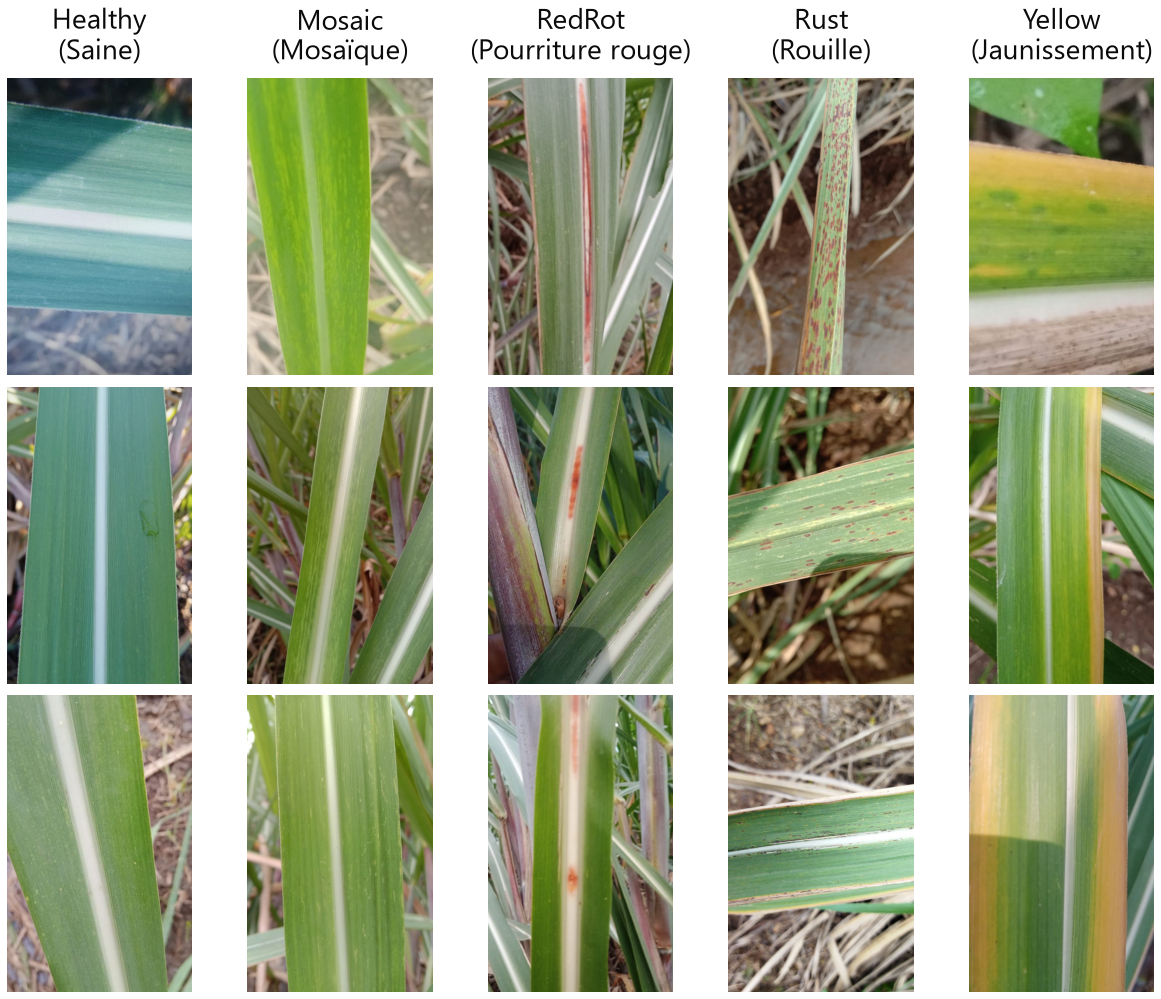
\includegraphics[width=0.92\textwidth]{dataset_samples.png}
\caption{Exemples d'images tirées au hasard pour chacune des cinq classes (recadrage d'affichage uniquement).}
\label{fig:samples}
\end{figure}

Les images ne sont ni uniformes ni normalisées : nous avons recensé 119 résolutions différentes, de $240\times292$ à $1600\times1600$ pixels. Deux formats portrait dominent, $493\times1040$ (958 images) et $780\times1040$ (580 images), ce qui donne un rapport largeur/hauteur médian de 0,56 (figure~\ref{fig:sizes}). Toutes les images sont en couleurs (RVB) et aucune n'est corrompue.

\begin{figure}[htbp]
\centering
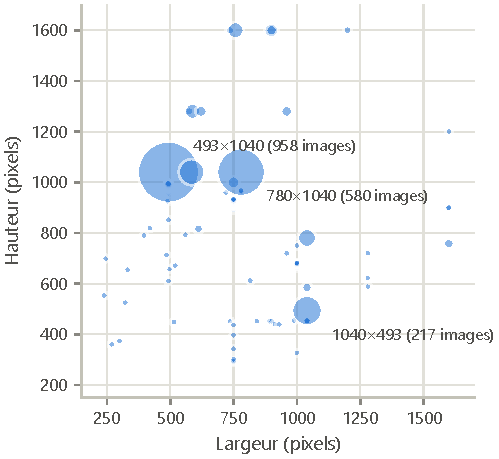
\includegraphics[width=0.52\textwidth]{image_sizes.pdf}
\caption{Résolutions des images brutes. La surface de chaque disque est proportionnelle au nombre d'images ayant cette résolution.}
\label{fig:sizes}
\end{figure}

\subsubsection{Audit et nettoyage}

Avant d'entraîner quoi que ce soit, nous avons calculé l'empreinte MD5 de chaque fichier. Le résultat a été une vraie surprise : \textbf{210 images sont des copies exactes} d'autres images (184 groupes de doublons). Elles se concentrent dans trois classes : 86 copies pour Mosaic (soit 18,6\,\% de la classe), 67 pour Rust et 46 pour Healthy. Aucun doublon ne relie deux classes différentes, il ne s'agit donc pas d'erreurs d'étiquetage. Le danger est ailleurs : avec un découpage aléatoire, une image et sa copie peuvent tomber l'une dans l'apprentissage, l'autre dans le test, et le modèle est alors évalué sur des images qu'il a déjà vues. Aucun des articles que nous avons consultés et qui utilisent ce jeu de données ne mentionne ce problème.

Nous avons ensuite cherché les quasi-doublons, c'est-à-dire la même photographie légèrement recadrée ou ré-encodée. Chaque image est réduite à une vignette $32\times32$ en niveaux de gris, centrée et réduite, puis comparée à toutes les autres par corrélation. Au-delà d'une corrélation de 0,90, toutes les paires examinées visuellement correspondaient à la même scène, prise deux fois ou recadrée de quelques pixels, et toujours dans la même classe ; en dessous de 0,85 apparaissaient au contraire des paires de feuilles différentes, simplement semblables par leur composition. Nous avons donc retenu le seuil de 0,90 et conservé une seule image par groupe, ce qui retire 24 images supplémentaires. Le jeu final compte \textbf{2\,287 images} (figure~\ref{fig:cleaning} et tableau~\ref{tab:dataset}).

\begin{figure}[htbp]
\centering
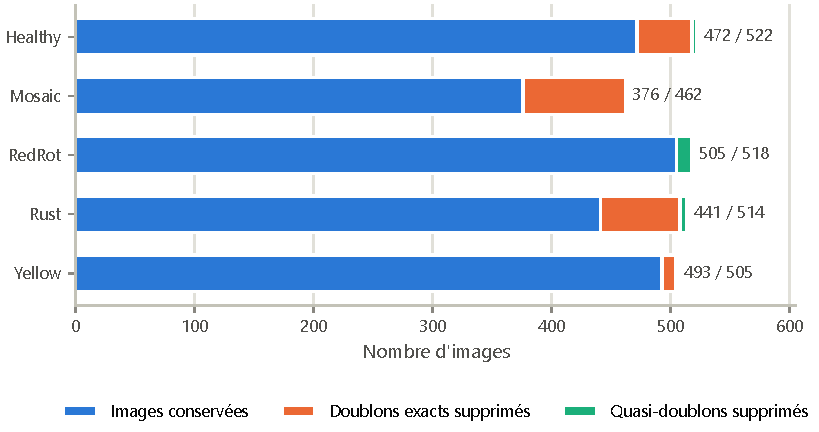
\includegraphics[width=0.8\textwidth]{class_distribution.pdf}
\caption{Effet du nettoyage sur chaque classe : images conservées et images supprimées (doublons exacts et quasi-doublons). Les nombres indiquent les images conservées sur le total initial.}
\label{fig:cleaning}
\end{figure}

\subsubsection{Répartition apprentissage, validation et test}

Le découpage est stratifié, afin que chaque sous-ensemble conserve les proportions des classes. On isole d'abord \textbf{15\,\% des images pour le test} (344 images), qui ne seront utilisées qu'une seule fois, à la fin. Les 1\,943 images restantes sont réparties en \textbf{cinq plis stratifiés} : à tour de rôle, chaque pli sert à la validation (environ 389 images) pendant que les quatre autres servent à l'apprentissage (environ 1\,554 images). Chaque modèle est donc entraîné cinq fois, ce qui donne une répartition d'environ 68\,\% pour l'apprentissage, 17\,\% pour la validation et 15\,\% pour le test. Le tableau~\ref{tab:dataset} détaille les effectifs ; les autres plis ne diffèrent du premier que d'une image au plus par classe.

\begin{table}[htbp]
\centering
\caption{Effectifs par classe avant et après nettoyage, et répartition pour le premier pli de la validation croisée.}
\label{tab:dataset}
\begin{tabular}{llrrrrr}
\toprule
\textbf{Classe} & \textbf{Nom français} & \textbf{Brut} & \textbf{Nettoyé} & \textbf{Apprentissage} & \textbf{Validation} & \textbf{Test} \\
\midrule
\tableinput{tables/dataset_table.tex}
\bottomrule
\end{tabular}
\end{table}

Après nettoyage, le jeu reste à peu près équilibré : la classe la plus petite (Mosaic, 376 images) représente 74\,\% de la plus grande (RedRot, 505 images). Ce léger déséquilibre ne justifie pas de pondérer la fonction de perte, mais il explique que nous rapportions des métriques moyennées par classe (moyenne \emph{macro}) en plus de l'accuracy.

\subsection{Prétraitement}
\label{sec:pretraitement}

Le prétraitement a deux rôles. Il met d'abord toutes les images au format que les réseaux attendent : une taille fixe et des valeurs d'intensité comparables à celles vues pendant le pré-entraînement. Il conditionne aussi la qualité de l'optimisation, car des entrées centrées et réduites stabilisent la descente de gradient et accélèrent la convergence \cite{ioffe2015batch}. Dans le cas des maladies des plantes, Barbedo rappelle que la variabilité des conditions d'acquisition (éclairage, cadrage, résolution) est l'une des principales sources d'erreur des systèmes automatiques \cite{barbedo2016review} ; un prétraitement uniforme limite au moins la part de cette variabilité qui ne relève pas des symptômes.

\paragraph{Redimensionnement.} Les images sont redimensionnées une fois pour toutes en $256\times256$ pixels (interpolation de Lanczos), puis ramenées à $224\times224$ à l'entrée du réseau, résolution à laquelle les quatre modèles pré-entraînés ont été conçus ou évalués. Ce redimensionnement ne conserve pas les proportions : une image portrait de $493\times1040$ est étirée horizontalement. Nous l'avons préféré à un recadrage central, qui aurait supprimé jusqu'à la moitié de la feuille, alors que les lésions (de pourriture rouge en particulier) se trouvent souvent vers les extrémités. La déformation est la même à l'apprentissage et au test, et les réseaux s'y adaptent sans difficulté. La version $256\times256$ est stockée sur disque au format PNG, sans perte, ce qui évite de redécoder les JPEG d'origine à chaque époque.

\paragraph{Normalisation.} Les intensités sont d'abord ramenées dans $[0,1]$, puis chaque canal $c$ est centré et réduit :
\begin{equation}
\tilde{x}_c = \frac{x_c - \mu_c}{\sigma_c}, \qquad c \in \{R, V, B\}.
\label{eq:norm}
\end{equation}
Pour les modèles pré-entraînés, nous reprenons les statistiques utilisées lors de leur pré-entraînement, faute de quoi les filtres appris recevraient des entrées décalées : $\mu=(0{,}485 ; 0{,}456 ; 0{,}406)$ et $\sigma=(0{,}229 ; 0{,}224 ; 0{,}225)$ pour MobileNetV4, ConvNeXtV2 et SE-ResNet-50, et $\mu=\sigma=(0{,}5 ; 0{,}5 ; 0{,}5)$ pour les poids d'EfficientNetV2 issus de l'implémentation TensorFlow d'origine. Pour le CNN entraîné from scratch, nous utilisons les statistiques de notre propre jeu, calculées sur l'ensemble de développement uniquement : $\mu=(0{,}499 ; 0{,}530 ; 0{,}382)$ et $\sigma=(0{,}193 ; 0{,}193 ; 0{,}199)$. Le canal bleu, nettement plus faible, reflète la dominante verte des images. Dans le code, cette normalisation est la première couche de chaque modèle : tous les modèles reçoivent ainsi exactement les mêmes images, ce qui simplifie aussi l'évaluation de la robustesse et les visualisations Grad-CAM.

\subsection{Augmentation de données}
\label{sec:augmentation}

Avec environ 1\,550 images d'apprentissage par pli, un réseau de plusieurs millions de paramètres finit par mémoriser les exemples. L'augmentation de données consiste à générer, à chaque époque, des variantes plausibles des images d'apprentissage, de façon à enseigner au modèle les invariances attendues (position, orientation, éclairage) sans collecter de nouvelles données \cite{shorten2019survey, perez2017effectiveness}. Elle agit comme un régulariseur et compte parmi les moyens les plus efficaces de limiter le surapprentissage sur de petits jeux de données.

Les transformations ont été choisies pour rester réalistes. Une feuille photographiée au champ peut apparaître à n'importe quelle position et dans n'importe quel sens, d'où le recadrage aléatoire, les symétries et une légère rotation. L'éclairage varie au cours de la journée, d'où les variations de luminosité et de contraste. En revanche, nous n'avons volontairement pas modifié la teinte et seulement très peu la saturation : la couleur est ici un symptôme (le jaune de la classe Yellow, le rouge de la classe RedRot), et la perturber reviendrait à brouiller l'information que le modèle doit apprendre. Concrètement, pour chaque image d'un lot, on tire indépendamment :
\begin{itemize}
  \item un recadrage aléatoire couvrant une fraction $a \sim \mathcal{U}(0{,}6 ; 1)$ de la surface, de rapport d'aspect $r$ tel que $\log r \sim \mathcal{U}(\log\tfrac{3}{4}, \log\tfrac{4}{3})$, placé au hasard dans l'image ;
  \item une rotation d'angle $\alpha \sim \mathcal{U}(-15^\circ, 15^\circ)$ ;
  \item une symétrie horizontale et une symétrie verticale, chacune avec une probabilité de 0,5 ;
  \item des facteurs de luminosité et de contraste dans $[0{,}75 ; 1{,}25]$ et un facteur de saturation dans $[0{,}85 ; 1{,}15]$.
\end{itemize}

Plutôt que d'enchaîner plusieurs opérations sur le processeur, les quatre transformations géométriques sont combinées en une seule transformation affine, appliquée sur GPU à tout le lot à la fois. Pour une image, les coordonnées normalisées $(u', v')$ du pixel de sortie sont envoyées vers les coordonnées $(u, v)$ de l'image source par
\begin{equation}
\begin{pmatrix} u \\ v \end{pmatrix} =
\begin{pmatrix} f_x\, s_x \cos\alpha & -f_y\, s_y \sin\alpha \\ f_x\, s_x \sin\alpha & f_y\, s_y \cos\alpha \end{pmatrix}
\begin{pmatrix} u' \\ v' \end{pmatrix} +
\begin{pmatrix} t_x \\ t_y \end{pmatrix},
\label{eq:affine}
\end{equation}
avec $s_x = \sqrt{a\,r}$ et $s_y=\sqrt{a/r}$ (tailles relatives du recadrage), $f_x, f_y \in \{-1, 1\}$ (symétries) et $t_x \sim (1-s_x)\,\mathcal{U}(-1,1)$, $t_y \sim (1-s_y)\,\mathcal{U}(-1,1)$ (position du recadrage). L'image est ensuite rééchantillonnée par interpolation bilinéaire ; les zones qui sortent de l'image source après rotation sont remplies par réflexion plutôt qu'en noir. Les modifications photométriques suivent, image par image, avec $g$ la luminance du pixel et $\bar{g}$ sa moyenne sur l'image :
\begin{equation}
x \leftarrow b\,x, \qquad x \leftarrow \bar{g} + c\,(x-\bar{g}), \qquad x \leftarrow g + s\,(x-g),
\label{eq:photo}
\end{equation}
chaque étape étant suivie d'un écrêtage dans $[0,1]$. L'augmentation n'est appliquée qu'aux images d'apprentissage ; les images de validation et de test sont seulement redimensionnées. Enfin, pour un pli donné, tous les modèles reçoivent les mêmes lots, dans le même ordre et avec les mêmes tirages aléatoires, puisque les générateurs sont initialisés avec la même graine. La figure~\ref{fig:augmentation} montre quelques variantes obtenues.

Ce choix d'implémentation a aussi une raison pratique. Sous Windows, les processus auxiliaires du chargeur de données de PyTorch démarrent lentement (chacun recharge toute la bibliothèque) et, au-delà de quelques-uns, leur démarrage échouait faute de mémoire virtuelle, ce qui bloquait l'entraînement. Garder les 2\,287 images en mémoire (environ 450~Mo) et faire l'augmentation sur GPU a supprimé le problème tout en accélérant les époques.

\begin{figure}[htbp]
\centering
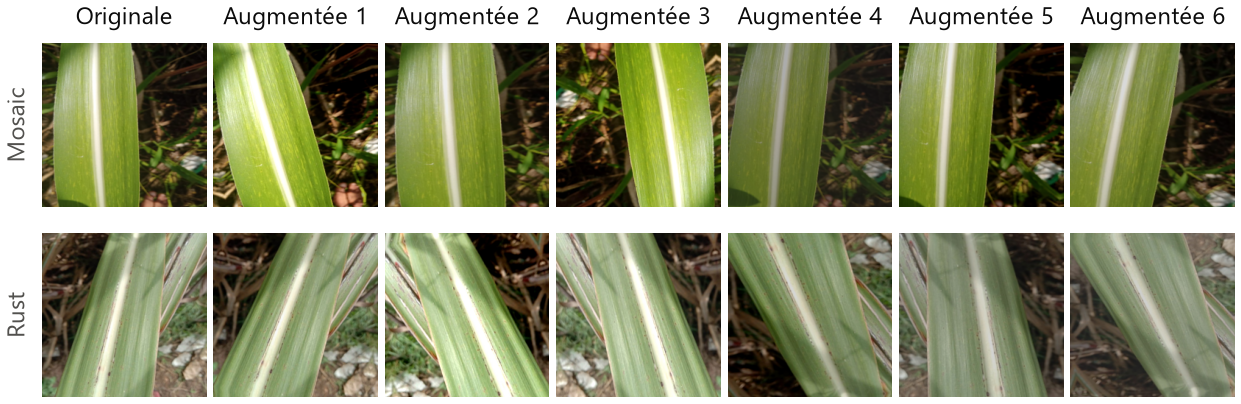
\includegraphics[width=\textwidth]{augmentation_examples.png}
\caption{Image d'origine et six variantes produites par l'augmentation, pour une feuille atteinte de mosaïque et une feuille atteinte de rouille.}
\label{fig:augmentation}
\end{figure}

\subsection{Modèles utilisés}
\label{sec:modeles}

\subsubsection{Architectures pré-entraînées}

Les quatre familles imposées par l'énoncé sont représentées par une variante de taille comparable, disponible avec des poids ImageNet-1k dans la bibliothèque \texttt{timm} \cite{wightman2019timm}.

\paragraph{EfficientNetV2-S \cite{tan2021efficientnetv2}.} EfficientNet \cite{tan2019efficientnet} a popularisé la mise à l'échelle conjointe de la profondeur, de la largeur et de la résolution d'un réseau de base obtenu par recherche d'architecture. La version~2 remplace, dans les premiers étages, les blocs MBConv (convolution en profondeur et module Squeeze-and-Excitation) par des blocs Fused-MBConv, où une convolution $3\times3$ classique se substitue à la paire expansion--convolution en profondeur, nettement plus rapide sur GPU. Elle a été conçue pour accélérer l'entraînement, avec une recherche d'architecture tenant compte du temps d'apprentissage et un apprentissage progressif où la taille des images et la régularisation augmentent au fil des époques ; les auteurs annoncent un entraînement jusqu'à quatre fois plus rapide que les modèles antérieurs, pour un nombre de paramètres jusqu'à 6,8 fois plus faible. Nous utilisons la variante S (\texttt{tf\_efficientnetv2\_s.in1k}).

\paragraph{MobileNetV4-Conv-M \cite{qin2024mobilenetv4}.} MobileNetV4 est la dernière génération de la famille MobileNet \cite{howard2019searching}, pensée pour les téléphones et les accélérateurs embarqués. Son bloc de base, l'\emph{Universal Inverted Bottleneck} (UIB), généralise le bloc inversé de MobileNetV2 en rendant optionnelles deux convolutions en profondeur, ce qui permet à la recherche d'architecture de choisir, étage par étage, le compromis le plus efficace pour le matériel visé. Nous utilisons la variante convolutive moyenne (\texttt{mobilenetv4\_conv\_medium.e500\_r224\_in1k}), la plus légère des quatre.

\paragraph{ConvNeXtV2-T \cite{woo2023convnextv2}.} ConvNeXt \cite{liu2022convnet} a montré qu'un réseau purement convolutif, modernisé avec des recettes issues des Vision Transformers (convolutions en profondeur $7\times7$, LayerNorm, activation GELU, goulot d'étranglement inversé), pouvait rivaliser avec eux. ConvNeXtV2 ajoute une couche de \emph{Global Response Normalization} (GRN), qui renforce la compétition entre canaux, et un pré-entraînement auto-supervisé par masquage (FCMAE) suivi d'un fine-tuning supervisé. Nous utilisons la variante Tiny (\texttt{convnextv2\_tiny.fcmae\_ft\_in1k}).

\paragraph{SE-ResNet-50 \cite{hu2018squeeze}.} Les réseaux Squeeze-and-Excitation (SENet) ajoutent à chaque bloc résiduel de ResNet \cite{he2016deep} un mécanisme d'attention par canal : les cartes de caractéristiques sont résumées par une moyenne globale (\emph{squeeze}), passées dans deux couches entièrement connectées, la première réduisant le nombre de canaux d'un facteur 16, puis dans une sigmoïde (\emph{excitation}), et le vecteur obtenu repondère les canaux. SENet a remporté la compétition de classification ILSVRC 2017 avec une erreur top-5 de 2,251\,\%. Nous utilisons SE-ResNet-50 (\texttt{seresnet50.ra2\_in1k}), le représentant le plus classique de la famille.

\subsubsection{CNN entraîné from scratch}

Pour mesurer ce qu'apporte réellement le pré-entraînement, nous avons conçu un CNN simple, de type VGG, initialisé aléatoirement (initialisation de He) et entraîné uniquement sur nos images. Il comporte une convolution d'entrée de pas 2, puis quatre blocs de deux convolutions $3\times3$ (chacune suivie d'une normalisation par lot et d'une ReLU) terminés par un sous-échantillonnage maximal (tableau~\ref{tab:scratch}). Avec 1,18 million de paramètres, il est volontairement compact : un réseau plus gros aurait surappris encore plus vite sur 1\,550 images. Sa sortie est, comme pour les autres modèles, une carte $7\times7$, ce qui permet de lui appliquer Grad-CAM de la même façon.

\begin{table}[htbp]
\centering
\caption{Architecture du CNN entraîné from scratch (entrée $3\times224\times224$).}
\label{tab:scratch}
\begin{tabular}{lccr}
\toprule
\textbf{Bloc} & \textbf{Couches} & \textbf{Sortie} & \textbf{Paramètres} \\
\midrule
Entrée & normalisation (statistiques du jeu) & $3\times224\times224$ & 0 \\
Tige & conv $3\times3$, pas 2, BN, ReLU & $32\times112\times112$ & 928 \\
Bloc 1 & $2\times$[conv $3\times3$, BN, ReLU], max-pool & $32\times56\times56$ & 18\,560 \\
Bloc 2 & $2\times$[conv $3\times3$, BN, ReLU], max-pool & $64\times28\times28$ & 55\,552 \\
Bloc 3 & $2\times$[conv $3\times3$, BN, ReLU], max-pool & $128\times14\times14$ & 221\,696 \\
Bloc 4 & $2\times$[conv $3\times3$, BN, ReLU], max-pool & $256\times7\times7$ & 885\,760 \\
Tête & moyenne globale, LayerNorm, dropout, linéaire & 5 & 1\,797 \\
\midrule
\textbf{Total} & & & \textbf{1\,184\,293} \\
\bottomrule
\end{tabular}
\end{table}

\subsubsection{Justification des choix}

Ces modèles couvrent trois aspects qui nous semblaient importants. Ils sont populaires et récents (2018 pour SENet, 2021 pour EfficientNetV2, 2023 pour ConvNeXtV2, 2024 pour MobileNetV4), ce qui permet de situer des architectures de 2023 et 2024, encore peu évaluées sur ce problème, par rapport à des références plus anciennes. Ils reposent sur des philosophies de conception différentes : architecture trouvée par recherche automatique et optimisée pour l'entraînement, architecture pensée pour le matériel mobile, réseau convolutif modernisé et pré-entraîné de manière auto-supervisée, et attention par canal ajoutée à un ResNet. Enfin, ils couvrent une large gamme de complexités, de 8,4 à 27,9 millions de paramètres et de 1,7 à 8,9~GFLOPs (tableau~\ref{tab:models}), ce qui permet de poser la question du compromis entre précision et coût.

Un point mérite d'être précisé : nous avons pris pour les quatre modèles des poids entraînés sur ImageNet-1k uniquement, alors que \texttt{timm} propose aussi des versions pré-entraînées sur ImageNet-21k (14 millions d'images) pour certaines architectures. Mélanger les deux aurait avantagé certains modèles pour une raison qui n'a rien à voir avec leur architecture.

\begin{table}[htbp]
\centering
\caption{Caractéristiques des modèles comparés, avec la tête de classification à cinq classes. Les GFLOPs sont mesurés pour une image $224\times224$ (une multiplication-addition compte pour deux opérations). L'accuracy top-1 sur ImageNet-1k est celle publiée par \texttt{timm} pour les poids utilisés, à 224 pixels (300 pour EfficientNetV2-S, qui n'est pas évalué à 224).}
\label{tab:models}
\small
\begin{tabular}{lccccc}
\toprule
\textbf{Modèle} & \textbf{Année} & \makecell{\textbf{Paramètres}\\\textbf{(M)}} & \textbf{GFLOPs} & \makecell{\textbf{Dimension de}\\\textbf{l'embedding}} & \makecell{\textbf{Top-1}\\\textbf{ImageNet (\%)}} \\
\midrule
EfficientNetV2-S & 2021 & 20,19 & 5,70 & 1\,280 & 83,2 \\
MobileNetV4-Conv-M & 2024 & 8,44 & 1,65 & 1\,280 & 79,1 \\
ConvNeXtV2-T & 2023 & 27,87 & 8,91 & 768 & 82,9 \\
SE-ResNet-50 & 2018 & 26,05 & 8,18 & 2\,048 & 80,3 \\
\midrule
CNN from scratch & -- & 1,18 & 1,52 & 256 & -- \\
\bottomrule
\end{tabular}
\end{table}

\subsubsection{Tête de classification commune}

Chaque réseau pré-entraîné est privé de son classifieur ImageNet. Sa sortie, une carte de caractéristiques, est résumée par une moyenne globale (le vecteur obtenu est appelé \emph{embedding} dans la suite), puis passée dans une tête identique pour tous les modèles : une normalisation LayerNorm, un dropout de taux 0,2 et une couche linéaire vers les cinq classes. Nous sommes arrivés à cette tête commune après un premier essai instructif. Avec la tête par défaut de \texttt{timm}, l'extraction de caractéristiques donnait des résultats curieusement faibles pour EfficientNetV2 et MobileNetV4 (moins de 70\,\% pour ce dernier sur le premier pli), avec une perte initiale supérieure à 8. L'explication tenait à l'initialisation : pour ces deux familles, les poids du classifieur sont tirés uniformément dans $\pm 1/\sqrt{K}$, où $K$ est le nombre de classes. C'est raisonnable pour les 1\,000 classes d'ImageNet ($\pm 0{,}03$), beaucoup moins pour nos 5 classes ($\pm 0{,}45$) : les logits de départ sont énormes et, le réseau étant gelé, il faut des centaines d'itérations pour les ramener à une échelle normale. La tête commune, avec l'initialisation standard de PyTorch, supprime ce biais et garantit que les différences observées viennent bien des représentations apprises.

\subsubsection{Stratégies d'apprentissage par transfert}
\label{sec:strategies}

Yosinski et al. ont montré que les premières couches d'un CNN apprennent des détecteurs génériques (contours, textures) qui se transfèrent bien, alors que les couches profondes deviennent de plus en plus spécifiques à la tâche d'origine \cite{yosinski2014transferable}. D'où trois façons d'adapter un réseau pré-entraîné, que nous comparons pour chaque architecture :
\begin{itemize}
  \item \textbf{Extraction de caractéristiques (FE)} : tout le réseau est gelé, y compris les statistiques des couches de normalisation par lot, et seule la tête est apprise. Le réseau sert d'extracteur fixe d'embeddings \cite{razavian2014cnn}.
  \item \textbf{Fine-tuning partiel (PFT)} : on dégèle le dernier étage du réseau, c'est-à-dire tous les blocs qui travaillent à la résolution la plus faible (cartes $7\times7$ pour une entrée $224\times224$), ainsi que les couches pré-entraînées situées entre cet étage et la tête (couche de projection de MobileNetV4, normalisation finale de ConvNeXtV2). Les étages précédents restent gelés.
  \item \textbf{Fine-tuning complet (FFT)} : tous les poids sont ré-entraînés.
\end{itemize}

Le tableau~\ref{tab:trainable} donne la part de paramètres entraînables dans chaque cas. Elle peut surprendre pour le fine-tuning partiel : le dernier étage concentre de 56 à 81\,\% des paramètres, parce que c'est là que le nombre de canaux est le plus élevé. Il ne représente pourtant qu'une petite partie de la profondeur (3 blocs sur 16 pour SE-ResNet-50, 3 sur 18 pour ConvNeXtV2) et une part encore plus faible du calcul, puisqu'il opère sur des cartes $7\times7$. En fine-tuning partiel, la rétropropagation s'arrête donc tôt, ce qui réduit le temps d'entraînement et la mémoire nécessaire.

Dans les deux variantes de fine-tuning, nous appliquons des taux d'apprentissage différenciés \cite{howard2018universal} : $10^{-3}$ pour la tête, initialisée aléatoirement, et $10^{-4}$ pour les couches pré-entraînées, afin de ne pas détruire trop vite ce qu'elles ont appris sur ImageNet. Les couches de normalisation par lot qui appartiennent à une partie gelée restent en mode évaluation : leurs moyennes et variances ne sont pas mises à jour.

\begin{table}[htbp]
\centering
\caption{Nombre de paramètres entraînables selon la stratégie (en millions, et en pourcentage du total).}
\label{tab:trainable}
\small
\begin{tabular}{lccc}
\toprule
\textbf{Modèle} & \makecell{\textbf{Extraction de}\\\textbf{caractéristiques (FE)}} & \makecell{\textbf{Fine-tuning}\\\textbf{partiel (PFT)}} & \makecell{\textbf{Fine-tuning}\\\textbf{complet (FFT)}} \\
\midrule
EfficientNetV2-S & 0,009 (0,05\,\%) & 14,90 (73,8\,\%) & 20,19 (100\,\%) \\
MobileNetV4-Conv-M & 0,009 (0,11\,\%) & 6,82 (80,8\,\%) & 8,44 (100\,\%) \\
ConvNeXtV2-T & 0,005 (0,02\,\%) & 15,49 (55,6\,\%) & 27,87 (100\,\%) \\
SE-ResNet-50 & 0,014 (0,05\,\%) & 16,56 (63,6\,\%) & 26,05 (100\,\%) \\
\bottomrule
\end{tabular}
\end{table}

\subsubsection{Fusion de caractéristiques}
\label{sec:fusion}

Les quatre architectures n'ont ni la même structure ni le même pré-entraînement : on peut donc espérer qu'elles ne se trompent pas sur les mêmes images et que leurs représentations se complètent. Deux grandes familles de fusion existent \cite{snoek2005early}. La \textbf{fusion précoce}, ou fusion au niveau des caractéristiques, combine les représentations avant la décision ; c'est l'approche retenue par plusieurs travaux sur les maladies des plantes, qui concatènent les caractéristiques profondes de deux réseaux ou plus \cite{khan2018ccdf, ji2020unitedmodel, sutaji2022lemoxinet}. La \textbf{fusion tardive}, ou fusion des décisions, combine les sorties de modèles entraînés séparément, par vote majoritaire ou moyenne des probabilités \cite{turkoglu2022plantdiseasenet}.

Pour la fusion précoce, notons $\phi_m(x)$ l'embedding produit par le réseau $m$ pour l'image $x$. Les embeddings de $M$ réseaux sont normalisés séparément puis concaténés, et un classifieur linéaire est appris sur le vecteur obtenu :
\begin{gather}
\mathbf{z}(x) = \Big[\, \mathrm{LN}_1\big(\phi_1(x)\big) \;\|\; \mathrm{LN}_2\big(\phi_2(x)\big) \;\|\; \cdots \;\|\; \mathrm{LN}_M\big(\phi_M(x)\big) \Big], \label{eq:fusion}\\
\hat{\mathbf{p}}(x) = \mathrm{softmax}\big(W\,\mathrm{Dropout}(\mathbf{z}(x)) + \mathbf{b}\big). \label{eq:fusion-head}
\end{gather}
La normalisation par branche (LayerNorm) est indispensable : sans elle, une branche dont les valeurs sont plus grandes, ou plus nombreuses (2\,048 dimensions pour SE-ResNet-50 contre 768 pour ConvNeXtV2), dominerait le vecteur fusionné. Avec $M=1$, cette tête est exactement la tête commune décrite plus haut.

Nous évaluons cette fusion avec deux sources d'embeddings : les réseaux pré-entraînés sur ImageNet, gelés (fusion de type FE), et les réseaux issus du fine-tuning complet sur le même pli (fusion de type FFT). Dans ce second cas, les réseaux n'ont vu que les images d'apprentissage du pli considéré, ce qui exclut toute fuite vers la validation ou le test. Comme les réseaux restent gelés, nous suivons le protocole classique en deux temps : les embeddings sont extraits une seule fois, sans augmentation, puis la tête de fusion est entraînée avec exactement les mêmes hyperparamètres que les autres modèles. Ce protocole rend le calcul assez léger pour tester les \textbf{15 combinaisons possibles} des quatre réseaux (4 seuls, 6 paires, 4 triplets, 1 quadruplet) sur les cinq plis.

Pour la fusion tardive, nous calculons le vote souple des quatre modèles fine-tunés, c'est-à-dire la moyenne de leurs probabilités :
\begin{equation}
\hat{\mathbf{p}}(x) = \frac{1}{M}\sum_{m=1}^{M} \mathbf{p}_m(x).
\label{eq:late}
\end{equation}

\subsection{Paramètres d'entraînement}
\label{sec:parametres}

L'énoncé insiste sur ce point : tous les modèles doivent être entraînés dans les mêmes conditions. Le tableau~\ref{tab:hyper} récapitule les réglages, communs à tous les modèles, à toutes les stratégies et à toutes les têtes de fusion. Nous ne les avons pas optimisés modèle par modèle : il s'agit de valeurs courantes pour le fine-tuning, fixées avant les expériences, ce qui évite de favoriser un modèle par un réglage plus soigné.

\begin{table}[htbp]
\centering
\caption{Hyperparamètres communs à toutes les expériences.}
\label{tab:hyper}
\small
\begin{tabularx}{0.92\textwidth}{l X}
\toprule
\textbf{Paramètre} & \textbf{Valeur} \\
\midrule
Résolution d'entrée & $224\times224$ \\
Taille de lot (batch size) & 32 \\
Nombre d'époques & 30 \\
Optimiseur & AdamW \cite{loshchilov2019decoupled}, $\beta_1=0{,}9$, $\beta_2=0{,}999$ \\
Taux d'apprentissage, nouvelles couches & $10^{-3}$ \\
Taux d'apprentissage, couches pré-entraînées & $10^{-4}$ \\
Ordonnancement & échauffement linéaire (2 époques) puis décroissance cosinus \\
Décroissance des poids (weight decay) & 0,05 \\
Fonction de perte & entropie croisée avec lissage des étiquettes $\varepsilon=0{,}1$ \\
Dropout de la tête & 0,2 \\
Précision numérique & mixte (bfloat16) \\
Sélection du modèle & meilleure accuracy de validation (à égalité : plus faible perte) \\
Validation croisée & 5 plis stratifiés, graine $42+k$ pour le pli $k$ \\
\bottomrule
\end{tabularx}
\end{table}

\paragraph{Optimiseur.} AdamW \cite{loshchilov2019decoupled} est une variante d'Adam \cite{kingma2015adam} dans laquelle la décroissance des poids est découplée de la mise à jour par le gradient, ce qui la rend plus efficace comme régularisation. C'est l'optimiseur de référence pour le fine-tuning des architectures récentes comme ConvNeXt.

\paragraph{Taux d'apprentissage.} Pendant les deux premières époques, le taux d'apprentissage croît linéairement de zéro jusqu'à sa valeur nominale $\eta_0$, ce qui évite que les gradients, encore désordonnés au début, ne dégradent les poids pré-entraînés. Il décroît ensuite selon une demi-période de cosinus \cite{loshchilov2017sgdr}. Avec $T$ le nombre total d'itérations et $T_w$ celui de l'échauffement :
\begin{equation}
\eta(t) =
\begin{cases}
\eta_0\, \dfrac{t+1}{T_w} & \text{si } t < T_w,\\[2mm]
\dfrac{\eta_0}{2}\left(1 + \cos\left(\pi\,\dfrac{t - T_w}{T - T_w}\right)\right) & \text{sinon.}
\end{cases}
\label{eq:lr}
\end{equation}

\paragraph{Taille de lot et nombre d'époques.} Un lot de 32 images tient en mémoire pour tous les modèles, y compris en fine-tuning complet, sur une carte graphique de 8~Go. Trente époques représentent environ 1\,450 itérations par entraînement ; les courbes d'apprentissage (section~\ref{sec:courbes}) montrent que c'est suffisant pour que tous les modèles convergent.

\paragraph{Régularisation.} Outre l'augmentation de données et le dropout \cite{srivastava2014dropout}, nous utilisons le lissage des étiquettes \cite{szegedy2016rethinking} : la cible n'est plus un vecteur \og un-parmi-$K$ \fg{} mais
\begin{equation}
q_k = (1-\varepsilon)\,\mathbb{1}[k=y] + \frac{\varepsilon}{K}, \qquad \mathcal{L} = -\sum_{k=1}^{K} q_k \log \hat{p}_k ,
\label{eq:ls}
\end{equation}
ce qui décourage le réseau de produire des probabilités trop proches de 0 ou de 1 et améliore en général la calibration.

\paragraph{Précision mixte.} Les calculs du réseau sont effectués en bfloat16 et la perte en float32 \cite{micikevicius2018mixed}, ce qui accélère l'entraînement sans perte de précision mesurable.

\paragraph{Validation croisée.} La validation croisée stratifiée à $k$ plis donne une estimation plus fiable et moins dépendante du hasard du découpage qu'une seule partition \cite{kohavi1995study}. Pour chacun des cinq plis, le modèle est entraîné sur quatre plis, l'époque retenue est celle qui maximise l'accuracy sur le pli restant, et le modèle obtenu est évalué sur l'ensemble de test, toujours le même. Chaque résultat est rapporté sous la forme moyenne $\pm$ écart-type sur les cinq plis. Au total, l'étude comprend 65 entraînements (4 architectures $\times$ 3 stratégies $\times$ 5 plis, plus 5 pour le CNN from scratch), auxquels s'ajoutent 150 têtes de fusion et 45 entraînements sur des sous-ensembles réduits de l'apprentissage, qui servent à mesurer le besoin en données (section~\ref{sec:efficacite-donnees}).

\subsection{Métriques d'évaluation}
\label{sec:metriques}

Pour une classe $k$, on compte les vrais positifs $TP_k$ (images de la classe $k$ correctement reconnues), les faux positifs $FP_k$ (images d'autres classes attribuées à tort à $k$), les faux négatifs $FN_k$ (images de $k$ attribuées à une autre classe) et les vrais négatifs $TN_k$. Les métriques suivantes en découlent \cite{sokolova2009systematic}.

\paragraph{Accuracy.} Proportion d'images correctement classées sur les $N$ images évaluées :
\begin{equation}
\mathrm{Accuracy} = \frac{1}{N}\sum_{i=1}^{N} \mathbb{1}\left[\hat{y}_i = y_i\right].
\end{equation}

\paragraph{Précision, rappel et F1-score.} La précision mesure la fiabilité d'une prédiction (parmi les images annoncées malades de $k$, combien le sont vraiment), le rappel mesure la capacité à retrouver toutes les images de la classe, et le F1-score est leur moyenne harmonique :
\begin{equation}
P_k = \frac{TP_k}{TP_k + FP_k}, \qquad R_k = \frac{TP_k}{TP_k + FN_k}, \qquad F1_k = \frac{2\,P_k\,R_k}{P_k + R_k}.
\end{equation}
Nous rapportons leur moyenne \emph{macro}, $P = \frac{1}{K}\sum_k P_k$ (et de même pour $R$ et $F1$), qui donne le même poids à chaque maladie quel que soit son effectif. En diagnostic, le rappel est souvent la métrique la plus importante : une maladie non détectée coûte généralement plus cher qu'une fausse alerte.

\paragraph{Matrice de confusion.} Tableau $K\times K$ dont la case $(i,j)$ compte les images de la classe réelle $i$ prédites dans la classe $j$. Nous la normalisons par ligne, si bien que la diagonale donne directement le rappel de chaque classe et que les cases hors diagonale montrent quelles maladies sont confondues entre elles.

\paragraph{Courbe ROC et AUC.} Pour une classe $k$ traitée en \og une contre toutes \fg{}, la courbe ROC trace le taux de vrais positifs $\mathrm{TPR}=TP_k/(TP_k+FN_k)$ en fonction du taux de faux positifs $\mathrm{FPR}=FP_k/(FP_k+TN_k)$ lorsque le seuil appliqué à la probabilité $\hat{p}_k$ varie de 1 à 0 \cite{fawcett2006introduction}. L'aire sous cette courbe,
\begin{equation}
\mathrm{AUC}_k = \int_{0}^{1} \mathrm{TPR}\; d(\mathrm{FPR}),
\end{equation}
s'interprète comme la probabilité qu'une image de la classe $k$, tirée au hasard, reçoive un score plus élevé qu'une image d'une autre classe. Contrairement à l'accuracy, elle ne dépend d'aucun seuil de décision. Nous rapportons l'AUC par classe et leur moyenne macro, qui est l'une des généralisations multiclasses de l'AUC discutées par Hand et Till \cite{hand2001simple}.

\paragraph{Coût et robustesse.} Pour répondre aux questions sur la légèreté et la robustesse des modèles, nous mesurons aussi le nombre de paramètres, le nombre d'opérations (GFLOPs), la latence d'inférence sur GPU et sur CPU, le temps d'entraînement et la mémoire GPU maximale. La robustesse est évaluée par l'accuracy sur des versions dégradées de l'ensemble de test (section~\ref{sec:robustesse}).

\section{Résultats obtenus}
\label{sec:resultats}

Sauf mention contraire, tous les résultats de cette section sont mesurés sur l'ensemble de test (344 images), qui n'a servi à aucun choix, et donnés sous la forme moyenne $\pm$ écart-type sur les cinq modèles issus de la validation croisée.

\subsection{Caractéristiques de l'unité de calcul}
\label{sec:materiel}

Toutes les expériences ont été menées sur un ordinateur portable dont le tableau~\ref{tab:hardware} décrit la configuration. Les entraînements ont été lancés les uns après les autres, jamais en parallèle, pour que les temps mesurés restent comparables, et tous utilisent les hyperparamètres du tableau~\ref{tab:hyper}. Les 65 entraînements principaux ont demandé 2~h~43 de calcul au total.

\begin{table}[htbp]
\centering
\caption{Environnement matériel et logiciel.}
\label{tab:hardware}
\small
\begin{tabularx}{0.92\textwidth}{l X}
\toprule
\textbf{Composant} & \textbf{Caractéristiques} \\
\midrule
Processeur & AMD Ryzen 9 8945HX (16 cœurs, 32 threads) \\
Carte graphique & NVIDIA GeForce RTX 5070 Laptop GPU, 8~Go de mémoire (architecture Blackwell) \\
Mémoire vive & 32~Go \\
Système d'exploitation & Windows 11 Pro \\
Langage & Python 3.12.13 \\
Apprentissage profond & PyTorch 2.14.1 (CUDA 13.0, cuDNN 9.24), torchvision 0.29.1, timm 1.0.31 \\
Analyse et figures & scikit-learn 1.9.1, NumPy 2.5.4, pandas 3.1.1, Matplotlib 3.11.2 \\
\bottomrule
\end{tabularx}
\end{table}

\subsection{Courbes d'apprentissage}
\label{sec:courbes}

La figure~\ref{fig:lc-fft} montre l'évolution de l'accuracy et de la perte au fil des époques en fine-tuning complet, en moyenne sur les cinq plis (la bande colorée correspond à $\pm$ un écart-type). Les quatre réseaux pré-entraînés convergent très vite : l'accuracy de validation dépasse 90\,\% dès la deuxième ou la troisième époque, et même dès la première pour ConvNeXtV2, puis se stabilise entre 97 et 99\,\% après une dizaine d'époques. L'accuracy d'apprentissage atteint presque 100\,\% et la perte d'apprentissage passe sous la perte de validation à partir de la cinquième époque environ. Il y a donc un léger surapprentissage, mais la perte de validation ne remonte jamais : la régularisation (augmentation, dropout, lissage des étiquettes, taux d'apprentissage réduit pour les couches pré-entraînées) suffit à le contenir. La perte ne descend pas sous 0,4 environ ; c'est l'effet attendu du lissage des étiquettes, qui empêche le modèle de viser une probabilité de 1.

Le CNN entraîné from scratch se comporte tout autrement. Il démarre autour de 50\,\%, progresse lentement et régulièrement, et atteint 94\,\% à la dernière époque, sans que l'écart entre apprentissage et validation ne se creuse. Ses courbes ne sont pas stabilisées après 30 époques : ce modèle souffre plutôt de sous-apprentissage et gagnerait sans doute quelques points avec un entraînement plus long. Nous avons préféré garder des conditions identiques pour tous les modèles, mais il faut garder cette limite en tête en lisant les comparaisons. Ses bandes d'écart-type, plus larges, traduisent aussi une plus grande sensibilité au pli.

\begin{figure}[htbp]
\centering
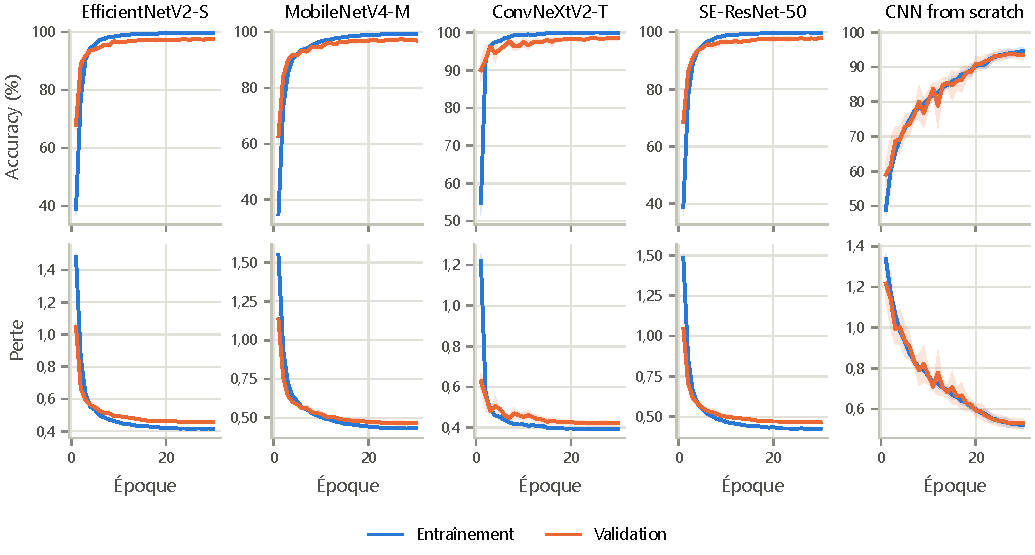
\includegraphics[width=\textwidth]{learning_curves_full_finetuning.pdf}
\caption{Courbes d'apprentissage en fine-tuning complet et pour le CNN from scratch (moyenne sur 5 plis, bande : $\pm$ un écart-type).}
\label{fig:lc-fft}
\end{figure}

En extraction de caractéristiques (figure~\ref{fig:lc-fe}), les courbes plafonnent bien plus bas, entre 84\,\% (MobileNetV4) et 91\,\% (EfficientNetV2-S, ConvNeXtV2 et SE-ResNet-50) en validation, et ce plafond est atteint vers la quinzième époque. La perte reste élevée, entre 0,6 et 0,75. Avec un réseau gelé, le modèle ne peut apprendre qu'une frontière linéaire dans l'espace des embeddings ImageNet, et cet espace sépare manifestement moins bien nos cinq classes. Le fine-tuning partiel (figure~\ref{fig:lc-pft}) a des courbes proches de celles du fine-tuning complet, avec un plateau un peu plus bas.

\begin{figure}[htbp]
\centering
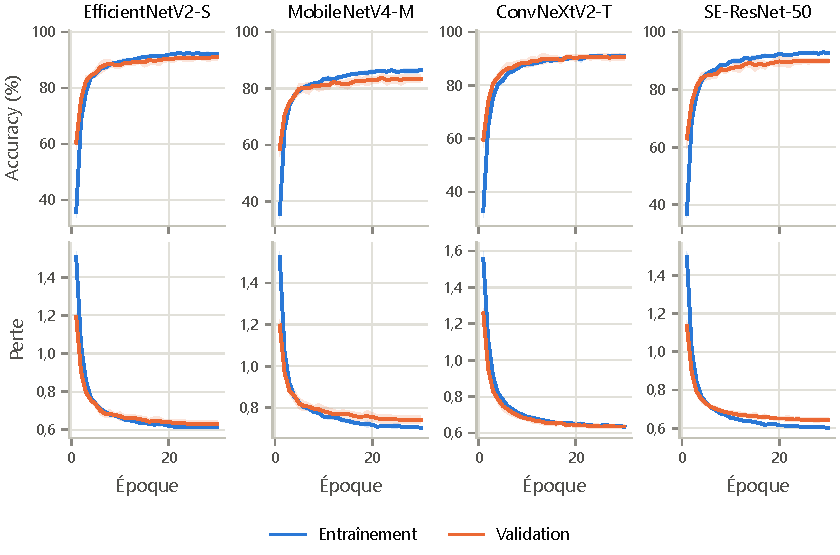
\includegraphics[width=0.9\textwidth]{learning_curves_feature_extraction.pdf}
\caption{Courbes d'apprentissage en extraction de caractéristiques (moyenne sur 5 plis).}
\label{fig:lc-fe}
\end{figure}

\begin{figure}[htbp]
\centering
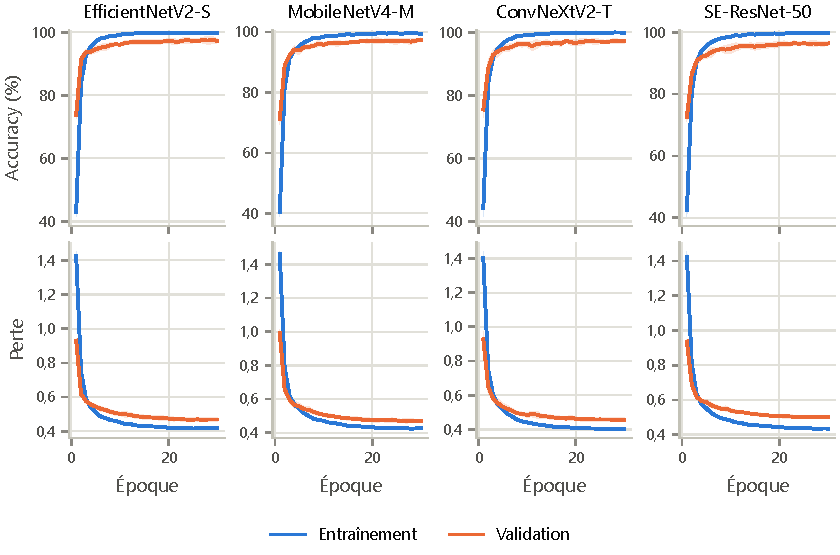
\includegraphics[width=0.9\textwidth]{learning_curves_partial_finetuning.pdf}
\caption{Courbes d'apprentissage en fine-tuning partiel (moyenne sur 5 plis).}
\label{fig:lc-pft}
\end{figure}

\subsection{Matrices de confusion}
\label{sec:confusion}

La figure~\ref{fig:confusion} présente les matrices de confusion des modèles en fine-tuning complet, du CNN from scratch et du modèle de fusion. Chacune cumule les prédictions des cinq modèles de la validation croisée sur l'ensemble de test (soit 1\,720 prédictions) et est normalisée par ligne : la diagonale donne le rappel de chaque classe, en pourcentage.

\begin{figure}[htbp]
\centering
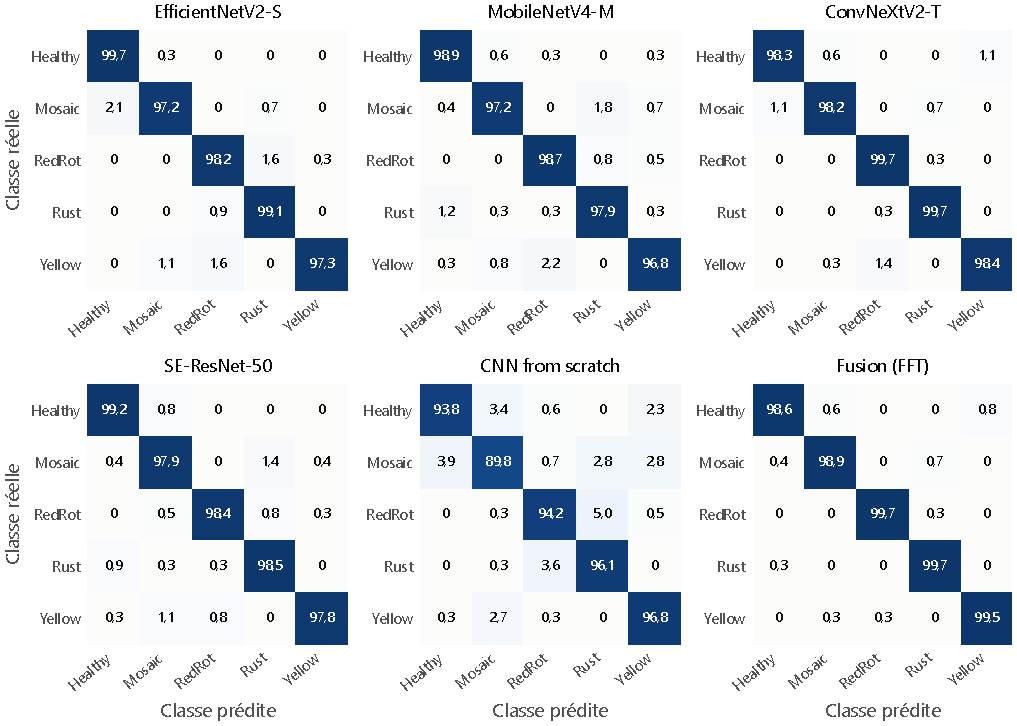
\includegraphics[width=\textwidth]{confusion_matrices.pdf}
\caption{Matrices de confusion normalisées par ligne (en \%), cumulées sur les cinq plis.}
\label{fig:confusion}
\end{figure}

Les erreurs des modèles pré-entraînés sont rares et se concentrent sur quelques paires de classes. Mosaic est la classe la plus difficile pour presque tous : son rappel varie de 97,2 à 98,2\,\% en fine-tuning complet et tombe à 89,8\,\% pour le CNN from scratch. Ses symptômes, des marbrures vert clair souvent discrètes, peuvent passer pour une feuille saine légèrement décolorée, d'où les confusions Mosaic $\rightarrow$ Healthy (2,1\,\% pour EfficientNetV2-S). C'est aussi la classe la plus réduite après nettoyage, avec 376 images. Deux autres confusions reviennent d'un modèle à l'autre : RedRot et Rust, qui présentent toutes deux des lésions brun-rouge allongées, et Yellow $\rightarrow$ RedRot (jusqu'à 2,2\,\% pour MobileNetV4), deux maladies qui modifient la couleur de la nervure centrale. Le CNN from scratch commet les mêmes types d'erreurs, mais bien plus souvent : 5,0\,\% des feuilles atteintes de pourriture rouge sont classées comme rouillées et 3,9\,\% des feuilles atteintes de mosaïque comme saines. Enfin, la fusion des embeddings fine-tunés (dernière matrice) réduit encore les confusions des modèles seuls : le rappel de Mosaic monte à 98,9\,\% et celui de Yellow à 99,5\,\%.

\subsection{Courbes ROC}
\label{sec:roc}

Les courbes ROC \og une classe contre toutes \fg{} (figure~\ref{fig:roc}) collent au coin supérieur gauche pour tous les modèles pré-entraînés ; il faut l'agrandissement de la région $\mathrm{FPR} \le 0{,}06$ pour voir des différences. On y retrouve la hiérarchie de la matrice de confusion : la courbe de la classe Mosaic est presque toujours la plus basse, et celles du CNN from scratch s'écartent nettement des autres.

\begin{figure}[htbp]
\centering
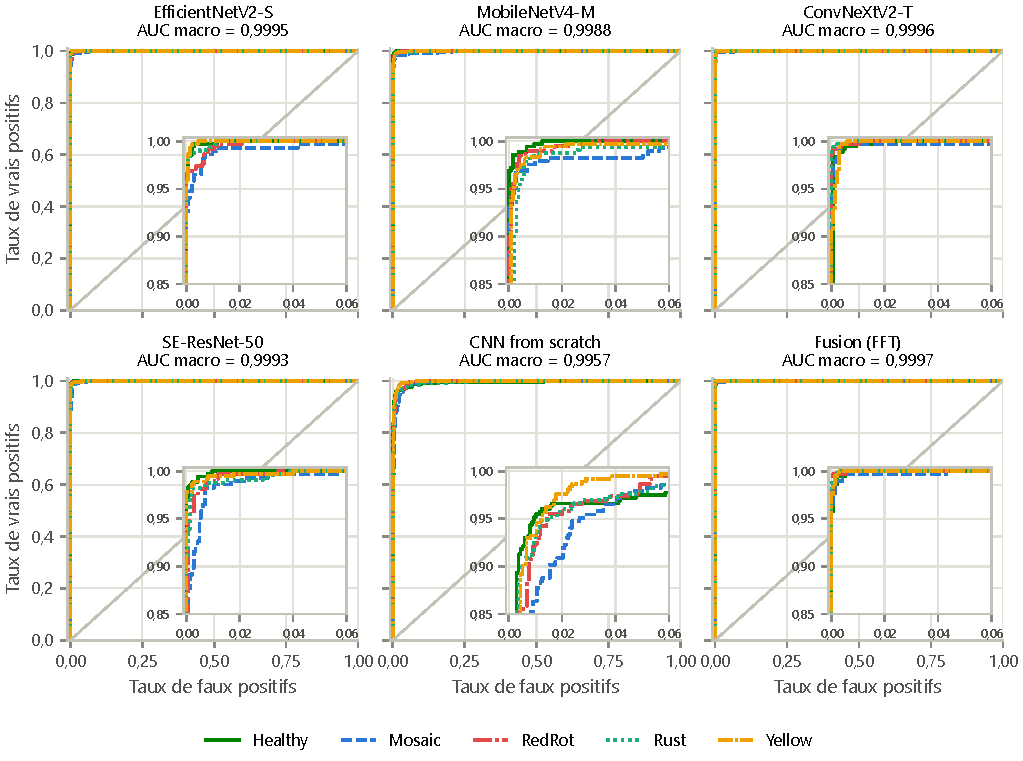
\includegraphics[width=\textwidth]{roc_curves.pdf}
\caption{Courbes ROC une classe contre toutes, calculées sur les prédictions cumulées des cinq plis. L'encart agrandit la région des faibles taux de faux positifs.}
\label{fig:roc}
\end{figure}

\subsection{AUC}
\label{sec:auc}

Le tableau~\ref{tab:auc} donne l'aire sous la courbe ROC pour chaque classe. Toutes les valeurs des modèles pré-entraînés dépassent 0,998, et la plupart 0,999 : lorsque ces modèles se trompent, ce n'est presque jamais avec assurance, puisque la bonne classe reçoit tout de même un score élevé. Même le CNN from scratch atteint 0,995 sur chaque classe, alors que son accuracy n'est que de 94\,\%. L'AUC est donc ici peu discriminante, et c'est surtout l'accuracy et le F1-score qui permettent de départager les modèles.

\begin{table}[htbp]
\centering
\caption{AUC par classe (une contre toutes), calculée sur les prédictions cumulées des cinq plis. En gras : meilleure valeur de chaque ligne.}
\label{tab:auc}
\small
\resizebox{\textwidth}{!}{%
\begin{tabular}{lccccccc}
\toprule
\textbf{Classe} & \textbf{EffNetV2-S} & \textbf{MNv4-M} & \textbf{ConvNeXtV2-T} & \textbf{SE-ResNet-50} & \textbf{Scratch} & \textbf{Fusion (FFT)} & \textbf{Vote souple} \\
\midrule
\tableinput{tables/results_per_class_auc.tex}
\bottomrule
\end{tabular}%
}
\end{table}

\subsection{Résultats globaux}
\label{sec:globaux}

Le tableau~\ref{tab:main} reprend le format demandé par l'énoncé, pour la meilleure stratégie de chaque architecture, le fine-tuning complet, ainsi que pour le CNN from scratch et les deux formes de fusion. Le tableau~\ref{tab:strategies} détaille ensuite les trois stratégies de transfert.

\begin{table}[htbp]
\centering
\caption{Résultats globaux sur l'ensemble de test (moyenne $\pm$ écart-type sur 5 plis). Précision, rappel et F1 sont des moyennes macro. Le temps est celui d'un entraînement complet (30 époques, validation comprise). $^{*}$ Pour les fusions, le nombre de paramètres et le temps incluent les quatre réseaux fine-tunés.}
\label{tab:main}
\small
\setlength{\tabcolsep}{4pt}
\resizebox{\textwidth}{!}{%
\begin{tabular}{lccccccc}
\toprule
\textbf{Modèle} & \textbf{Accuracy (\%)} & \textbf{Précision (\%)} & \textbf{Rappel (\%)} & \textbf{F1 (\%)} & \textbf{AUC} & \makecell{\textbf{Param.}\\\textbf{(M)}} & \makecell{\textbf{Temps}\\\textbf{d'entraîn.}} \\
\midrule
\tableinput{tables/results_main.tex}
\bottomrule
\end{tabular}%
}
\end{table}

\begin{table}[htbp]
\centering
\caption{Comparaison des stratégies de transfert. Accuracy de validation (pli de validation, utilisé pour choisir l'époque) et métriques de test. La mémoire est le pic d'occupation GPU pendant l'entraînement.}
\label{tab:strategies}
\footnotesize
\setlength{\tabcolsep}{3.5pt}
\resizebox{\textwidth}{!}{%
\begin{tabular}{llccccccc}
\toprule
\textbf{Modèle} & \textbf{Stratégie} & \makecell{\textbf{Param.}\\\textbf{entraînables}} & \makecell{\textbf{Acc. val.}\\\textbf{(\%)}} & \makecell{\textbf{Acc. test}\\\textbf{(\%)}} & \makecell{\textbf{F1 test}\\\textbf{(\%)}} & \textbf{AUC test} & \textbf{Temps} & \makecell{\textbf{Mémoire}\\\textbf{(Go)}} \\
\midrule
\tableinput{tables/results_strategies.tex}
\bottomrule
\end{tabular}%
}
\end{table}

Plusieurs enseignements ressortent de ces deux tableaux.

\paragraph{Le fine-tuning complet l'emporte pour toutes les architectures.} Avec $98{,}9 \pm 0{,}6$\,\% d'accuracy, ConvNeXtV2-T obtient le meilleur résultat, devant SE-ResNet-50 (98,4\,\%), EfficientNetV2-S (98,3\,\%) et MobileNetV4-M (97,9\,\%). Les quatre modèles tiennent en un point, un écart du même ordre que la variation d'un pli à l'autre (0,4 à 0,8 point). Pour savoir si ces différences sont réelles, nous avons estimé par bootstrap, avec 10\,000 rééchantillonnages des images de test, un intervalle de confiance à 95\,\% de l'écart avec le meilleur modèle (tableau~\ref{tab:significance}). Seuls MobileNetV4 ($-1{,}0$ point) et le CNN from scratch ($-4{,}6$ points) sont significativement en dessous de ConvNeXtV2 ; l'avance de ce dernier sur EfficientNetV2-S et SE-ResNet-50 n'est pas significative avec 344 images de test.

\begin{table}[htbp]
\centering
\caption{Accuracy de test et intervalle de confiance à 95\,\% obtenu par bootstrap sur les images de test (10\,000 tirages). L'écart est mesuré par rapport au meilleur modèle unique, ConvNeXtV2-T (une valeur positive signifie que le modèle fait mieux que lui) ; il est jugé significatif si son intervalle de confiance exclut zéro.}
\label{tab:significance}
\small
\resizebox{\textwidth}{!}{%
\begin{tabular}{lccccc}
\toprule
\textbf{Modèle} & \textbf{Accuracy (\%)} & \textbf{IC 95\,\%} & \makecell{\textbf{Écart avec}\\\textbf{ConvNeXtV2-T (points)}} & \textbf{IC 95\,\% de l'écart} & \textbf{Significatif} \\
\midrule
\tableinput{tables/results_significance.tex}
\bottomrule
\end{tabular}%
}
\end{table}

\paragraph{Le niveau de fine-tuning compte davantage que l'architecture.} Passer de l'extraction de caractéristiques au fine-tuning complet fait gagner entre 7,6 points (SE-ResNet-50) et 14,0 points (MobileNetV4), alors que les quatre architectures ne diffèrent que d'un point une fois fine-tunées (figure~\ref{fig:strategies}). Le fine-tuning partiel se place entre les deux. Il récupère l'essentiel du gain pour EfficientNetV2-S (97,2\,\%), mais reste 3,4 points sous le fine-tuning complet pour ConvNeXtV2 (95,5\,\%), alors qu'il entraîne déjà 56\,\% de ses paramètres. Ré-entraîner le seul dernier étage ne suffit donc pas : les étages intermédiaires, qui encodent des textures et des motifs de taille moyenne, doivent eux aussi s'adapter à des lésions foliaires très différentes des objets d'ImageNet. Le fine-tuning partiel garde en revanche l'avantage du coût : pour ConvNeXtV2, il prend 2~minutes au lieu de 5 et occupe 0,83~Go de mémoire GPU au lieu de 3,85.

\begin{figure}[htbp]
\centering
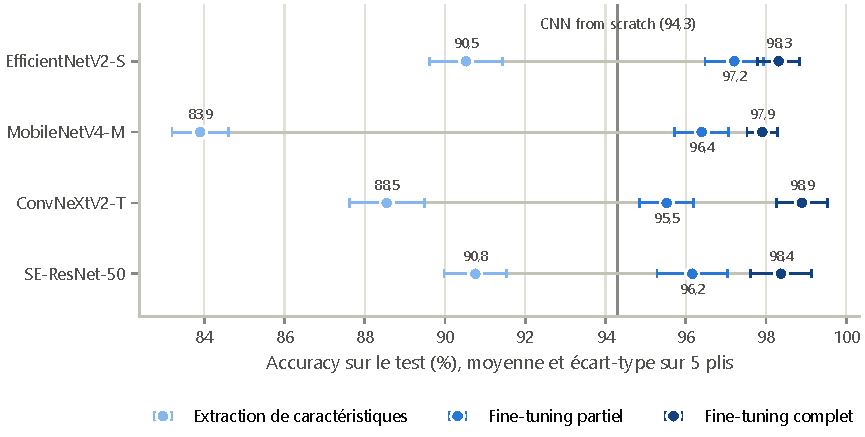
\includegraphics[width=0.9\textwidth]{strategy_comparison.pdf}
\caption{Accuracy de test selon la stratégie de transfert (moyenne et écart-type sur 5 plis). La ligne verticale grise indique le CNN entraîné from scratch.}
\label{fig:strategies}
\end{figure}

\paragraph{Un petit CNN from scratch fait mieux que l'extraction de caractéristiques.} Résultat plus inattendu, notre CNN de 1,2 million de paramètres (94,3\,\%) dépasse toutes les variantes en extraction de caractéristiques (83,9 à 90,8\,\%). Les caractéristiques ImageNet gelées, apprises pour distinguer des chiens, des voitures ou des oiseaux, ne séparent pas linéairement des différences aussi fines que celles qui distinguent une feuille saine d'une feuille atteinte de mosaïque ; un réseau, même modeste, qui adapte toutes ses couches à la tâche s'en sort mieux. Le transfert redevient nettement gagnant dès qu'on autorise le fine-tuning : avec ConvNeXtV2, le taux d'erreur passe de 5,7\,\% à 1,1\,\%, soit cinq fois moins d'erreurs, et le modèle est beaucoup plus stable d'un pli à l'autre (écart-type de 0,6 point contre 2,1).

\paragraph{La validation est un peu optimiste pour les stratégies partielles.} En fine-tuning complet, l'accuracy de validation et celle de test sont très proches. En extraction de caractéristiques et en fine-tuning partiel, la validation surestime parfois le test, jusqu'à 2,6 points pour ConvNeXtV2. L'époque retenue étant choisie sur le pli de validation, cette mesure est légèrement biaisée vers le haut ; c'est précisément pour cela qu'il fallait un ensemble de test qui n'intervienne dans aucun choix.

\paragraph{Performances par maladie.} Le tableau~\ref{tab:perclass} donne le F1-score de chaque classe. En fine-tuning complet, toutes les classes dépassent 97\,\% pour les quatre réseaux, et ConvNeXtV2 dépasse 98,5\,\% sur les cinq. Mosaic reste la classe la plus faible pour la plupart des modèles, et l'écart avec les autres classes se creuse fortement pour le CNN from scratch (90,6\,\%).

\begin{table}[htbp]
\centering
\caption{F1-score par classe (en \%), calculé sur les prédictions cumulées des cinq plis. En gras : meilleure valeur de chaque ligne.}
\label{tab:perclass}
\small
\resizebox{\textwidth}{!}{%
\begin{tabular}{lccccccc}
\toprule
\textbf{Classe} & \textbf{EffNetV2-S} & \textbf{MNv4-M} & \textbf{ConvNeXtV2-T} & \textbf{SE-ResNet-50} & \textbf{Scratch} & \textbf{Fusion (FFT)} & \textbf{Vote souple} \\
\midrule
\tableinput{tables/results_per_class_f1.tex}
\bottomrule
\end{tabular}%
}
\end{table}

\subsection{Fusion de caractéristiques}
\label{sec:resultats-fusion}

Le tableau~\ref{tab:fusion} et la figure~\ref{fig:fusion} présentent la fusion des embeddings pour les 15 combinaisons possibles des quatre réseaux, à partir des réseaux gelés (embeddings ImageNet) et des réseaux issus du fine-tuning complet. Dans les deux cas, seule la tête de fusion est entraînée, sur des embeddings extraits une fois pour toutes, sans augmentation. Les lignes à un seul réseau servent de référence dans ce même protocole ; pour les embeddings ImageNet, elles retrouvent à un point près les résultats de l'extraction de caractéristiques du tableau~\ref{tab:strategies}, ce qui montre que l'absence d'augmentation ne change pas les conclusions.

\begin{table}[htbp]
\centering
\caption{Fusion des embeddings (accuracy et F1 de test, en \%, moyenne $\pm$ écart-type sur 5 plis). E : EfficientNetV2-S, M : MobileNetV4-M, C : ConvNeXtV2-T, S : SE-ResNet-50. La dernière ligne donne le vote souple des quatre modèles fine-tunés. En gras : meilleure accuracy de chaque colonne.}
\label{tab:fusion}
\small
\begin{tabular}{clcccc}
\toprule
& & \multicolumn{2}{c}{\textbf{Embeddings ImageNet (gelés)}} & \multicolumn{2}{c}{\textbf{Embeddings fine-tunés}} \\
\cmidrule(lr){3-4}\cmidrule(lr){5-6}
\textbf{$M$} & \textbf{Réseaux fusionnés} & \textbf{Accuracy} & \textbf{F1} & \textbf{Accuracy} & \textbf{F1} \\
\midrule
\tableinput{tables/results_fusion.tex}
\bottomrule
\end{tabular}
\end{table}

\paragraph{Sur des réseaux gelés, la fusion aide sans remplacer le fine-tuning.} Avec les embeddings ImageNet, le meilleur réseau seul (EfficientNetV2-S, 91,1\,\%) est dépassé par la fusion des quatre, qui atteint $92{,}7 \pm 0{,}5$\,\%, soit 1,6 point de mieux avec un écart-type deux fois plus faible. Le gain plafonne dès trois réseaux. Détail intéressant, MobileNetV4, le plus faible seul (84,1\,\%), fait partie de l'un des deux meilleurs triplets (M + C + S) : ses représentations, bien que moins discriminantes, apportent une information que les autres n'ont pas. Mais même la meilleure fusion de réseaux gelés reste cinq points en dessous du moins bon modèle fine-tuné : juxtaposer plusieurs représentations génériques ne remplace pas l'adaptation des réseaux au domaine.

\paragraph{Sur des réseaux fine-tunés, la fusion donne le meilleur résultat de l'étude.} Les embeddings issus du fine-tuning complet sont déjà très discriminants : une simple tête linéaire réentraînée dessus retrouve les performances des modèles d'origine (99,0\,\% pour ConvNeXtV2). La fusion les améliore encore : 99,1\,\% pour les meilleures paires, 99,2\,\% pour le meilleur triplet et $99{,}3 \pm 0{,}6$\,\% pour les quatre réseaux. Le vote souple des quatre modèles fine-tunés, qui ne demande aucun apprentissage supplémentaire, fait aussi bien ($99{,}4 \pm 0{,}5$\,\%) ; la différence entre les deux fusions n'est pas significative. Toutes deux réduisent d'environ moitié le taux d'erreur du meilleur modèle seul, qui passe de 1,1\,\% à 0,6\,\%, et leur avance sur ConvNeXtV2 (+0,4 et +0,5 point) est significative dans les deux cas (tableau~\ref{tab:significance}).

\begin{figure}[htbp]
\centering
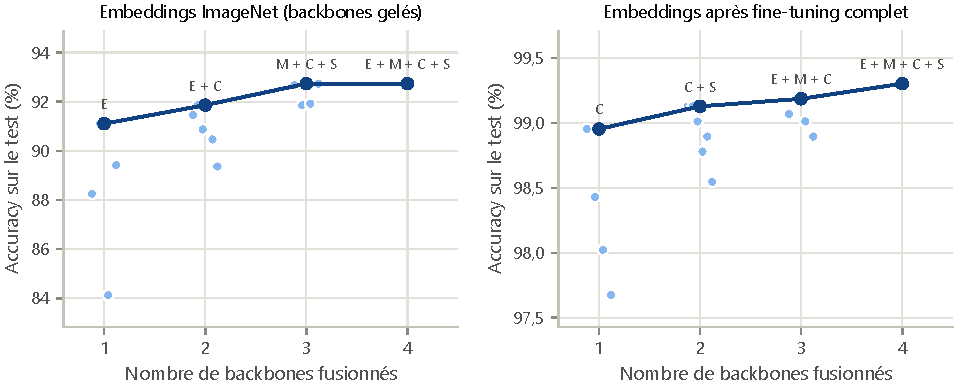
\includegraphics[width=0.95\textwidth]{fusion_gain.pdf}
\caption{Accuracy de test selon le nombre de réseaux fusionnés. Chaque point clair est une combinaison ; la ligne foncée relie la meilleure combinaison de chaque taille.}
\label{fig:fusion}
\end{figure}

Ce gain a un prix. La fusion des quatre réseaux mobilise 82,6 millions de paramètres et environ 24,4~GFLOPs par image, soit trois fois plus que ConvNeXtV2 seul, et suppose d'entraîner quatre modèles. Elle se justifie pour un service d'analyse centralisé, où chaque erreur évitée compte ; elle se justifie beaucoup moins sur un téléphone.

\subsection{Analyse comparative}
\label{sec:analyse}

\subsubsection{Quel modèle est le plus précis ?}
\label{sec:precision}

Parmi les modèles uniques, ConvNeXtV2-T en fine-tuning complet est le plus précis, avec $98{,}9 \pm 0{,}6$\,\% d'accuracy et un F1 macro de 98,9\,\%, mais son avance sur SE-ResNet-50 et EfficientNetV2-S n'est pas significative. Les deux fusions font mieux encore (99,3 et 99,4\,\%) et sont les seules à battre ConvNeXtV2 de façon significative. Pour la précision pure, sans contrainte de calcul, il faut donc retenir le vote souple des quatre modèles fine-tunés ; pour un modèle unique, ConvNeXtV2-T. Notons que le classement ne suit pas celui d'ImageNet : EfficientNetV2-S, le meilleur des quatre sur ImageNet (tableau~\ref{tab:models}), n'est que troisième ici, ce qui rappelle qu'avec quatre modèles seulement et des écarts aussi faibles, la corrélation observée par Kornblith et al. \cite{kornblith2019better} ne peut pas servir de règle de choix.

\subsubsection{Quel modèle est le plus léger ?}
\label{sec:legerete}

Le tableau~\ref{tab:efficiency} et la figure~\ref{fig:efficiency} comparent le coût des modèles en inférence. MobileNetV4-M est de loin le plus léger des réseaux pré-entraînés : 8,4 millions de paramètres (32~Mo en float32) et 1,65~GFLOPs par image, soit trois à cinq fois moins que les autres. Sur le processeur, il classe une image en 30~ms, contre 64 à 97~ms pour les autres réseaux, et c'est aussi le plus rapide à entraîner (2~min~21~s par pli) et le moins gourmand en mémoire GPU (0,94~Go). Il ne perd qu'un point d'accuracy par rapport à ConvNeXtV2 (97,9 contre 98,9\,\%), ce qui en fait le meilleur candidat pour une application sur téléphone.

\begin{table}[htbp]
\centering
\caption{Coût des modèles en inférence (entrée $224\times224$). Latence mesurée image par image (lot de 1), sur GPU en bfloat16 et sur CPU en float32 avec 4 threads ; débit mesuré sur GPU avec des lots de 32 images.}
\label{tab:efficiency}
\small
\begin{tabular}{lcccccc}
\toprule
\textbf{Modèle} & \makecell{\textbf{Paramètres}\\\textbf{(M)}} & \makecell{\textbf{Taille}\\\textbf{(Mo)}} & \textbf{GFLOPs} & \makecell{\textbf{Latence}\\\textbf{GPU (ms)}} & \makecell{\textbf{Débit GPU}\\\textbf{(images/s)}} & \makecell{\textbf{Latence}\\\textbf{CPU (ms)}} \\
\midrule
\tableinput{tables/results_efficiency.tex}
\bottomrule
\end{tabular}
\end{table}

Sur GPU, la hiérarchie est différente et mérite une remarque. Avec une seule image à la fois, la carte graphique est loin d'être saturée et la latence dépend surtout du nombre d'opérations à lancer les unes après les autres : ConvNeXtV2, avec ses 18 blocs, répond le plus vite (17~ms), alors qu'EfficientNetV2-S et ses 40 blocs, plus légers mais plus nombreux, mettent 50~ms. Dès que l'on traite des lots, le nombre d'opérations reprend le dessus et MobileNetV4 traite 1\,673 images par seconde, 2,6 fois plus que ConvNeXtV2. Le CNN from scratch est encore plus léger (1,2 million de paramètres, 12~ms sur CPU), mais il paie cette légèreté de près de cinq points d'accuracy. À l'autre extrémité, la fusion des quatre réseaux coûte environ trois fois plus que ConvNeXtV2 seul pour un demi-point de gain.

\begin{figure}[htbp]
\centering
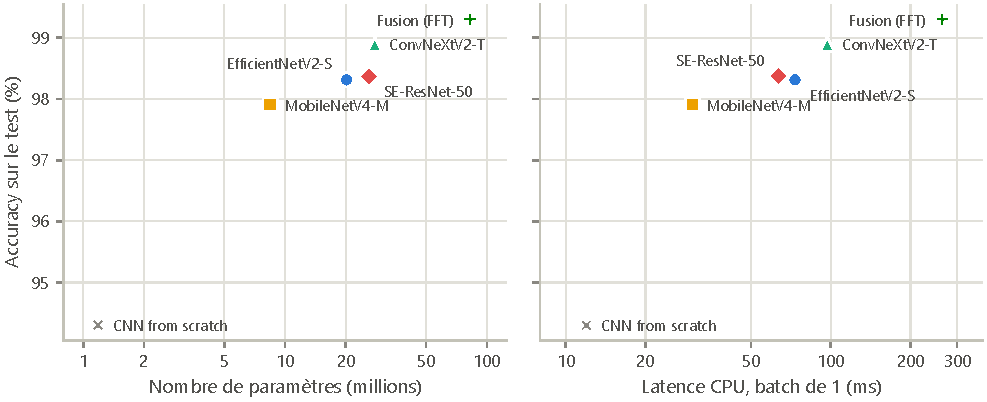
\includegraphics[width=\textwidth]{efficiency_tradeoff.pdf}
\caption{Compromis entre accuracy de test et coût d'inférence (axes horizontaux logarithmiques).}
\label{fig:efficiency}
\end{figure}

\subsubsection{Quel modèle est le plus robuste ?}
\label{sec:robustesse}

Une photo prise au champ avec un téléphone d'entrée de gamme est rarement parfaite : bruit de capteur en faible lumière, flou de bougé, sous-exposition, compression agressive à l'envoi, feuille partiellement masquée. Pour mesurer la robustesse des modèles à ces défauts, nous avons dégradé l'ensemble de test de cinq façons, à trois niveaux de sévérité, sans jamais montrer ces dégradations aux modèles pendant l'apprentissage : bruit gaussien d'écart-type $\sigma \in \{0{,}04 ; 0{,}08 ; 0{,}12\}$, flou gaussien ($\sigma \in \{1 ; 2 ; 3\}$ pixels), assombrissement (intensités multipliées par 0,7, 0,5 ou 0,3), compression JPEG (qualité 30, 15 ou 5) et occultation par un carré gris couvrant 25, 35 ou 45\,\% du côté de l'image, placé au hasard. La figure~\ref{fig:robustness} et le tableau~\ref{tab:robustness} donnent les résultats.

\begin{figure}[htbp]
\centering
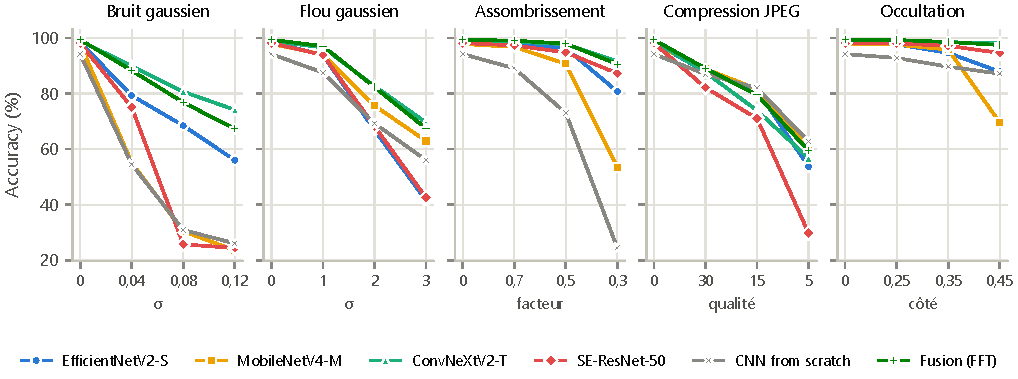
\includegraphics[width=\textwidth]{robustness.pdf}
\caption{Accuracy de test en fonction de la sévérité de la dégradation (moyenne sur 5 plis). Le niveau 0 correspond aux images d'origine.}
\label{fig:robustness}
\end{figure}

\begin{table}[htbp]
\centering
\caption{Robustesse aux dégradations : accuracy (en \%) sur les images d'origine, puis moyenne sur les trois niveaux de chaque dégradation, moyenne générale et baisse par rapport aux images d'origine. La colonne \og Original \fg{} est recalculée dans le même protocole (images requantifiées sur 8 bits), d'où de légers écarts avec le tableau~\ref{tab:main}.}
\label{tab:robustness}
\small
\setlength{\tabcolsep}{4.5pt}
\resizebox{\textwidth}{!}{%
\begin{tabular}{lcccccccc}
\toprule
\textbf{Modèle} & \textbf{Original} & \textbf{Bruit} & \textbf{Flou} & \makecell{\textbf{Assom-}\\\textbf{brissement}} & \textbf{JPEG} & \textbf{Occultation} & \textbf{Moyenne} & \textbf{Baisse} \\
\midrule
\tableinput{tables/results_robustness.tex}
\bottomrule
\end{tabular}%
}
\end{table}

Le constat principal est une grande disparité entre architectures, que l'accuracy sur images propres ne laissait pas deviner. Les quatre réseaux fine-tunés sont à moins d'un point les uns des autres sur les images d'origine, mais leur accuracy moyenne sur images dégradées va de 71,7\,\% (MobileNetV4) à 86,4\,\% (ConvNeXtV2). Le bruit gaussien est la dégradation la plus discriminante : au niveau le plus fort, ConvNeXtV2 conserve 74\,\% d'accuracy, alors que MobileNetV4 et SE-ResNet-50 tombent sous 25\,\%, à peine mieux que le hasard (20\,\%). Une forte compression JPEG (qualité 5) pénalise tous les modèles, tandis que l'occultation d'une partie de la feuille est bien tolérée, sauf au niveau le plus fort par MobileNetV4 (69,5\,\%) et, dans une moindre mesure, par EfficientNetV2-S (87,8\,\%). Le CNN from scratch est le plus fragile de tous (67,5\,\% en moyenne), en particulier face au bruit et à l'assombrissement.

Un second constat nous a surpris. Pour trois architectures sur quatre, le fine-tuning partiel est nettement plus robuste que le fine-tuning complet, alors qu'il est moins précis sur images propres : 81,2 contre 71,7\,\% en moyenne pour MobileNetV4, 80,6 contre 72,1\,\% pour SE-ResNet-50 et 83,6 contre 78,9\,\% pour EfficientNetV2-S. Une explication plausible est qu'en ré-entraînant tout le réseau sur des images propres, on spécialise aussi ses premiers filtres, ceux qui, appris sur la diversité d'ImageNet, étaient les plus tolérants au bruit ; en les gelant, le fine-tuning partiel conserve cette tolérance. ConvNeXtV2 fait exception : son fine-tuning complet est à la fois le plus précis et le plus robuste.

La réponse à la question posée est donc claire : parmi les modèles uniques, \textbf{ConvNeXtV2-T est le plus robuste}, avec la plus forte accuracy moyenne sous dégradation et la plus faible baisse (12,5 points). Le vote souple des quatre modèles fait encore un peu mieux (87,5\,\%, baisse de 11,9 points). La robustesse au changement de données d'apprentissage, mesurée par l'écart-type entre plis, départage moins les modèles : les quatre réseaux fine-tunés varient de 0,4 à 0,8 point d'un pli à l'autre, MobileNetV4 étant le plus régulier, alors que le CNN from scratch varie de 2,1 points.

\subsubsection{Quel est le besoin en données ?}
\label{sec:efficacite-donnees}

Pour vérifier que l'apprentissage par transfert réduit réellement le besoin en données, nous avons ré-entraîné ConvNeXtV2-T et MobileNetV4-M en fine-tuning complet, ainsi que le CNN from scratch, sur 10, 25 et 50\,\% des images d'apprentissage de chaque pli, tirées au hasard en respectant les proportions des classes. Les hyperparamètres, le pli de validation et l'ensemble de test sont inchangés. La figure~\ref{fig:data-efficiency} et le tableau~\ref{tab:data-efficiency} donnent les résultats.

\begin{figure}[htbp]
\centering
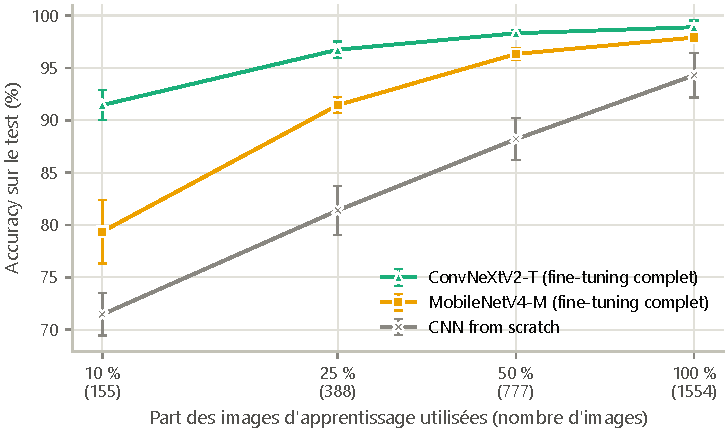
\includegraphics[width=0.8\textwidth]{data_efficiency.pdf}
\caption{Accuracy de test selon la part des images d'apprentissage utilisées (moyenne et écart-type sur 5 plis ; axe horizontal logarithmique). Entre parenthèses : nombre moyen d'images d'apprentissage par pli.}
\label{fig:data-efficiency}
\end{figure}

\begin{table}[htbp]
\centering
\caption{Accuracy de test (en \%) selon la part des images d'apprentissage utilisées, avec le nombre moyen d'images entre parenthèses (moyenne $\pm$ écart-type sur 5 plis).}
\label{tab:data-efficiency}
\small
\begin{tabular}{lcccc}
\toprule
\textbf{Modèle} & \textbf{10\,\% (155)} & \textbf{25\,\% (388)} & \textbf{50\,\% (777)} & \textbf{100\,\% (1\,554)} \\
\midrule
\tableinput{tables/results_data_efficiency.tex}
\bottomrule
\end{tabular}
\end{table}

L'avantage du pré-entraînement grandit à mesure que les données se raréfient. Avec seulement 155 images d'apprentissage, une trentaine par classe, ConvNeXtV2 reconnaît encore 91,5\,\% des images de test, alors que le CNN from scratch tombe à 71,5\,\% : vingt points d'écart, contre 4,6 avec toutes les données. Plus parlant encore, ConvNeXtV2 entraîné sur un quart des images (388) fait mieux (96,7\,\%) que le CNN from scratch entraîné sur la totalité (94,3\,\%), et avec la moitié des images il n'est plus qu'à 0,6 point de son score final. MobileNetV4 profite moins du pré-entraînement quand les données sont très rares (79,4\,\% avec 10\,\% des images, avec un écart-type de 3 points), ce qui suggère que ses représentations, plus compactes et optimisées pour la vitesse, se transfèrent moins bien avec très peu d'exemples ; l'écart avec ConvNeXtV2 se résorbe presque entièrement à partir de la moitié des données. Le CNN from scratch, enfin, progresse encore nettement entre 50 et 100\,\% des images : c'est lui qui profiterait le plus d'un jeu de données plus grand.

\section{Interprétabilité du modèle}
\label{sec:interpretabilite}

Une accuracy élevée ne dit pas \emph{pourquoi} le modèle a raison. Sur des photographies prises au champ, un réseau peut très bien s'appuyer sur des indices sans rapport avec la maladie : la couleur du sol, la présence de feuilles sèches en arrière-plan, l'heure de la prise de vue, voire le téléphone utilisé. Un tel modèle obtiendrait de bons scores sur un test issu de la même campagne d'acquisition et échouerait ailleurs. Pour un outil destiné à des agriculteurs, il est donc important de vérifier que les décisions reposent bien sur les symptômes.

\subsection{Principe de Grad-CAM}

Grad-CAM \cite{selvaraju2017gradcam}, qui généralise la méthode CAM \cite{zhou2016learning}, produit une carte de chaleur indiquant les régions de l'image qui ont le plus contribué au score d'une classe. Soit $A^k \in \mathbb{R}^{H\times W}$ la $k$-ième carte de caractéristiques de la dernière couche convolutive et $y^c$ le score (avant softmax) de la classe $c$. On calcule d'abord l'importance de chaque carte en moyennant le gradient du score sur toutes les positions :
\begin{equation}
\alpha_k^c = \frac{1}{H\,W} \sum_{i=1}^{H}\sum_{j=1}^{W} \frac{\partial y^c}{\partial A^k_{ij}},
\label{eq:gradcam-weights}
\end{equation}
puis on combine les cartes pondérées en ne gardant que les contributions positives :
\begin{equation}
L^c_{\text{Grad-CAM}} = \mathrm{ReLU}\left( \sum_{k} \alpha_k^c\, A^k \right).
\label{eq:gradcam}
\end{equation}
La ReLU élimine les régions qui font baisser le score de la classe, qui relèvent plutôt des autres classes. La carte obtenue a la résolution de la dernière couche, ici $7\times7$ pour les cinq modèles ; elle est agrandie à $224\times224$ par interpolation bilinéaire, normalisée entre 0 et 1, puis superposée à l'image. Nous calculons la carte pour la classe prédite, avec les modèles du premier pli.

Cette résolution de $7\times7$ est la principale limite de la méthode : chaque cellule couvre environ $32\times32$ pixels de l'image d'entrée, si bien que Grad-CAM localise des \emph{régions} et non des lésions individuelles. Elle suffit néanmoins pour savoir si le modèle regarde la feuille ou l'arrière-plan, et quelle partie de la feuille.

\section{Discussion}
\label{sec:discussion}

\subsection{Forces}

\paragraph{Des performances élevées.} XX

\paragraph{Un faible besoin en données.} XX

\paragraph{La réutilisation des connaissances pré-entraînées.} XX

\paragraph{Un protocole qui limite les biais.} L'audit du jeu de données, l'ensemble de test isolé et la validation croisée à cinq plis rendent nos chiffres plus fiables qu'un découpage aléatoire unique. Les mêmes hyperparamètres, les mêmes lots et les mêmes tirages d'augmentation pour tous les modèles font que les écarts observés tiennent bien aux architectures et aux stratégies. Enfin, la tête commune a évité un biais discret, mais réel, lié à l'initialisation des classifieurs de \texttt{timm}.

\subsection{Limites}

\paragraph{Un jeu de données acquis dans des conditions homogènes.} Toutes les images proviennent de quelques exploitations d'un même district indien, ont été prises en août et septembre, par temps clair, avec trois téléphones \cite{daphal2023enhancing}. La plupart sont des gros plans d'une seule feuille, cadrée par un opérateur. Les modèles n'ont donc vu ni d'autres variétés, ni d'autres saisons, ni des conditions de lumière difficiles, ni des feuilles photographiées de loin au milieu du couvert végétal.

\paragraph{Une généralisation non vérifiée en conditions réelles.} Notre ensemble de test est tiré du même jeu de données que l'apprentissage. Il mesure la capacité à reconnaître de nouvelles photos prises dans les mêmes conditions, pas la capacité à fonctionner dans un autre contexte. L'expérience de Mohanty et al., dont le modèle passait de 99\,\% à environ 31\,\% sur des images d'une autre origine \cite{mohanty2016using}, montre que l'écart peut être considérable. Les tests de robustesse de la section~\ref{sec:robustesse} donnent une première indication, mais ils ne remplacent pas un vrai jeu de test externe, comme les 427 photos de terrain utilisées par Indra et al. \cite{indra2026sugarcane}.

\paragraph{Un léger déséquilibre des classes.} Le nettoyage a surtout réduit la classe Mosaic, qui ne compte plus que 376 images contre 505 pour RedRot. Ce déséquilibre reste modéré et les métriques macro montrent qu'il n'a pas pénalisé la classe minoritaire de façon visible, mais il pourrait compter davantage avec un jeu plus déséquilibré.

\paragraph{Une seule étiquette par image.} Chaque feuille est rangée dans une seule classe. Or une même feuille peut porter plusieurs maladies à la fois, ou une maladie à un stade très précoce difficile à distinguer d'une feuille saine. Les étiquettes du jeu n'ont pas été vérifiées par un second expert, et nous n'avons aucun moyen d'estimer leur taux d'erreur.

\paragraph{Une incertitude statistique non négligeable.} Avec 344 images de test, une différence d'un point d'accuracy correspond à trois ou quatre images. XX

\paragraph{Des choix méthodologiques discutables.} Le seuil de 0,90 utilisé pour les quasi-doublons a été fixé après inspection visuelle : des photographies d'une même feuille prises sous un angle un peu différent peuvent subsister dans des plis différents. Le redimensionnement sans conservation des proportions déforme les lésions. Enfin, un seul jeu d'hyperparamètres a été utilisé pour tous les modèles : c'est ce qui rend la comparaison équitable, mais certains modèles auraient sans doute gagné à un réglage spécifique, en particulier le CNN from scratch, pour qui 30 époques sont peu.

\paragraph{Une interprétabilité limitée.} Les cartes Grad-CAM ont une résolution de $7\times7$ et ne localisent que des régions. Elles indiquent où le modèle regarde, pas ce qu'il y reconnaît.

\subsection{Perspectives}

\paragraph{Apprentissage multimodal.} Une photographie ne dit pas tout : la variété cultivée, l'âge de la culture, la météo des jours précédents ou l'historique de la parcelle orientent fortement le diagnostic d'un agronome. Un modèle multimodal pourrait combiner l'image avec ces données tabulaires, ou avec d'autres capteurs. L'imagerie hyperspectrale, en particulier, permet de détecter certaines maladies avant l'apparition des symptômes visibles \cite{rumpf2010early, mahlein2016plant}. La fusion de caractéristiques étudiée ici en est un premier pas : le même principe de concaténation d'embeddings normalisés s'applique à des sources de nature différente.

\paragraph{Déploiement sur smartphone.} XX Il faudrait ensuite le convertir dans un format adapté au mobile (TensorFlow Lite, ONNX ou Core ML) et vérifier l'effet de la quantification, qui avait coûté plus de cinq points à Daphal et Koli \cite{daphal2024enhanced}. L'application pourrait fonctionner hors connexion, ce qui compte dans les zones rurales, et afficher la carte Grad-CAM pour que l'agriculteur voie sur quelle partie de la feuille repose le diagnostic.

\paragraph{Détection en temps réel par drone.} Pour surveiller de grandes surfaces, il faudrait passer de la classification de gros plans à la détection des zones malades dans des images aériennes. Cela suppose des modèles de détection ou de segmentation (de type YOLO, déjà utilisés pour la canne à sucre \cite{kumpala2022sugarcane, malik2021disease}), entraînés sur des images prises à plusieurs mètres de hauteur, où chaque feuille n'occupe que quelques dizaines de pixels. Les embeddings appris ici pourraient servir d'initialisation pour la partie classification d'un tel système.

\paragraph{Données et méthodes.} À plus court terme, plusieurs pistes permettraient de consolider nos conclusions : constituer un jeu de test externe, pris dans une autre région et avec d'autres téléphones ; fusionner les jeux publics existants, après dédoublonnage, comme l'ont fait Arman et al. \cite{arman2025sugarcaneshufflenet} ; pré-entraîner les réseaux de manière auto-supervisée sur des images agricoles non étiquetées ; distiller la connaissance du modèle de fusion dans MobileNetV4 pour cumuler précision et légèreté ; ajouter une classe \og autre \fg{} ou un seuil de confiance, pour que le modèle sache dire qu'il ne reconnaît pas une maladie absente de l'apprentissage.

\section{Conclusion}
\label{sec:conclusion}

\paragraph{Objectifs.} Ce projet visait à reconnaître automatiquement quatre maladies foliaires de la canne à sucre, ainsi que les feuilles saines, à partir de photographies prises au champ, et à mesurer ce qu'apporte l'apprentissage par transfert lorsque les données sont peu nombreuses : quelle architecture choisir, jusqu'où adapter un réseau pré-entraîné, et s'il est utile de combiner plusieurs réseaux.

\paragraph{Méthodologie.} Après avoir audité le jeu de données de Daphal et Koli et retiré 234 images redondantes, nous avons comparé quatre architectures récentes et de tailles différentes, EfficientNetV2-S, MobileNetV4-Conv-M, ConvNeXtV2-T et SE-ResNet-50, chacune selon trois stratégies (extraction de caractéristiques, fine-tuning partiel et fine-tuning complet), ainsi qu'un CNN entraîné from scratch. Tous les modèles ont été entraînés avec les mêmes hyperparamètres, les mêmes lots et les mêmes augmentations, puis évalués par validation croisée à cinq plis sur un ensemble de test isolé, avec un bootstrap pour juger de la significativité des écarts. Nous avons également étudié la fusion des embeddings des quatre réseaux sur toutes les combinaisons possibles, le vote souple, la robustesse aux dégradations d'image, le coût de calcul, le besoin en données et l'interprétation des décisions par Grad-CAM.

\paragraph{Meilleurs résultats.} Le fine-tuning complet de ConvNeXtV2-T donne le meilleur modèle unique, avec $98{,}9 \pm 0{,}6$\,\% d'accuracy, un F1 macro de 98,9\,\% et une AUC de 0,9998 ; c'est aussi le plus robuste aux dégradations et celui dont les cartes Grad-CAM suivent le mieux les lésions. La fusion des quatre réseaux fine-tunés, par concaténation des embeddings ou par vote souple, atteint 99,3 à 99,4\,\% et réduit de moitié environ le taux d'erreur, au prix d'un calcul trois fois plus lourd. Pour un usage sur téléphone, MobileNetV4-M offre le meilleur compromis : 97,9\,\% d'accuracy avec 8,4 millions de paramètres et 30~ms par image sur CPU, à condition de surveiller sa sensibilité au bruit.

\paragraph{Apport du transfer learning.} L'apprentissage par transfert est nettement gagnant, mais à une condition : il faut fine-tuner le réseau. Utilisés comme simples extracteurs de caractéristiques, les réseaux ImageNet plafonnent entre 84 et 91\,\%, en dessous d'un petit CNN entraîné from scratch (94,3\,\%). Une fois fine-tunés, ils divisent par cinq le nombre d'erreurs de ce CNN, convergent en quelques époques, résistent mieux aux dégradations d'image et concentrent leur attention sur les symptômes. Ils ont aussi besoin de beaucoup moins de données : avec un quart des images d'apprentissage, ConvNeXtV2 dépasse déjà le CNN from scratch entraîné sur la totalité, et avec 155 images seulement il conserve 91,5\,\% d'accuracy, contre 71,5\,\% pour ce dernier. Le pré-entraînement sur ImageNet apporte donc surtout un excellent point de départ, que le fine-tuning adapte ensuite aux textures et aux couleurs des lésions foliaires.

Ces résultats ont été obtenus sur un jeu de données acquis dans une seule région et dans des conditions assez homogènes. La prochaine étape consisterait à les confirmer sur des photographies prises ailleurs, avec d'autres téléphones et à d'autres saisons, avant d'envisager un déploiement de MobileNetV4 sur smartphone, puis le passage à la détection des maladies dans des images de drone.

\section*{Contributions}
\addcontentsline{toc}{section}{Contributions}
\label{sec:contributions}

Le projet a été réalisé individuellement. Le tableau~\ref{tab:contrib} détaille les tâches effectuées.

\begin{table}[htbp]
\centering
\caption{Répartition des tâches.}
\label{tab:contrib}
\begin{tabularx}{\textwidth}{>{\bfseries}l X}
\toprule
\textbf{Étudiant} & \textbf{Contribution} \\
\midrule
Abderrahmane EL-HOUIJ &
Recherche bibliographique et rédaction de l'état de l'art ; téléchargement, audit et nettoyage du jeu de données (doublons exacts et quasi-doublons) ; découpage stratifié et validation croisée ; implémentation du pipeline en PyTorch (prétraitement, augmentation sur GPU, tête commune, trois stratégies de transfert, CNN from scratch, fusion de caractéristiques et vote souple) ; entraînement des 65 modèles et des 150 têtes de fusion ; évaluation (métriques, matrices de confusion, courbes ROC, robustesse, coût de calcul) ; visualisations Grad-CAM ; rédaction du rapport et du fichier README ; organisation du dépôt Git. \\
\bottomrule
\end{tabularx}
\end{table}


\clearpage
\printbibliography[heading=bibintoc,title={Références}]

\appendix
\section{Organisation du code et reproduction des résultats}
\label{sec:annexe}

Le code source est disponible dans le dépôt \depot. Il est écrit en Python avec PyTorch et \texttt{timm}, et organisé en une série de scripts à exécuter dans l'ordre, qui s'appuient sur un petit paquet \texttt{src/} regroupant les éléments réutilisables.

\begin{table}[htbp]
\centering
\caption{Organisation du dépôt.}
\label{tab:repo}
\begin{tabularx}{\textwidth}{>{\ttfamily}l X}
\toprule
\textrm{\textbf{Fichier}} & \textbf{Rôle} \\
\midrule
src/config.py & chemins, classes, hyperparamètres et choix des modèles, regroupés en un seul endroit \\
src/data.py & lecture des images, découpage par pli, chargeur de lots et augmentation sur GPU \\
src/models.py & réseaux pré-entraînés, CNN from scratch, tête commune, stratégies de transfert, tête de fusion \\
src/engine.py & boucles d'entraînement et d'évaluation, ordonnancement du taux d'apprentissage \\
src/metrics.py & métriques globales et par classe, matrice de confusion, courbes ROC \\
src/gradcam.py & implémentation de Grad-CAM \\
src/plots.py & style commun des figures \\
\midrule
prepare\_data.py & téléchargement, audit (doublons), découpage stratifié, mise en cache $256\times256$ \\
explore\_data.py & figures et tableau de description du jeu de données \\
train.py & entraînement des 4 architectures $\times$ 3 stratégies et du CNN from scratch, sur les 5 plis ; option \texttt{--fractions} pour l'étude du besoin en données \\
train\_fusion.py & extraction des embeddings, têtes de fusion (15 combinaisons) et vote souple \\
benchmark.py & coût de calcul (paramètres, GFLOPs, latences) et robustesse aux dégradations \\
evaluate.py & agrégation des résultats, tableaux \LaTeX{} et figures du rapport \\
explain.py & cartes Grad-CAM \\
\bottomrule
\end{tabularx}
\end{table}

La reproduction complète tient en quelques commandes, après installation des dépendances listées dans \texttt{requirements.txt} (PyTorch avec prise en charge CUDA de préférence) :
\begin{verbatim}
python prepare_data.py --download
python explore_data.py
python train.py
python train_fusion.py
python benchmark.py
python train.py --models convnextv2_t mobilenetv4_m scratch_cnn \
                --strategies full_finetuning --fractions 0.1 0.25 0.5
python evaluate.py
python explain.py
\end{verbatim}
Sur notre machine, l'ensemble demande environ trois heures, dont l'essentiel pour \texttt{train.py}. Chaque entraînement terminé est enregistré (historique, prédictions, poids, résumé) et sauté si l'on relance le script, ce qui permet de reprendre un calcul interrompu. Les prédictions et les résumés de tous les entraînements sont versionnés dans le dépôt : \texttt{evaluate.py} peut donc régénérer les tableaux et la plupart des figures sans refaire les entraînements.


\end{document}
